% !Mode:: "TeX:UTF-8"
%%  本模板推荐以下方式编译:
%%
%%     1. PDFLaTeX[推荐]
%%  注意:
%%   1. 文件默认的编码为 UTF-8 对于windows,请选用支持UTF-8编码的编辑器。
%%   2. 若是模板有什么问题,请及时与我们取得联系,Email:latexstudio@qq.com。
%%   3. 可以到  https://wenda.latexstudio.net 提问
%%   4. 请安装 最新版本的 TeXLive 地址:https://www.latexstudio.net/page/texsoftware/

\documentclass{apmcmthesis}

\usepackage{url}
\usepackage{fontspec}
\defaultfontfeatures{Mapping=tex-text}
\usepackage{xunicode}
\usepackage{xltxtra}
%\setmainfont{???}
\usepackage{amsmath}
\usepackage{amsfonts}
\usepackage{amssymb}
\usepackage{graphicx}
\usepackage{array}
\usepackage{float}   %{H}
\usepackage{booktabs}  %\toprule[1.5pt]
%===================%插入代码需要的控制
\usepackage{listings}
\usepackage{xcolor}
\setmonofont{Consolas}%字体
\lstset{
	numbers=left, 
	numberstyle= \tiny, 
	keywordstyle= \color{ blue!70},
	commentstyle= \color{red!50!green!50!blue!50}, 
	frame=shadowbox, % 阴影效果
	rulesepcolor= \color{ red!20!green!20!blue!20} ,
	escapeinside=``,% 英文分号中可写入中文
	breaklines=true,
	basicstyle=\ttfamily 
} 
%===================%
%%%%%%%%%%%%填写相关信息%%%%%%%%%%%%%%%%%%%%%%%%%%
\tihao{A}                            %选题
\baominghao{2020220060005}           %报名号
\begin{document}

\pagestyle{frontmatterstyle}
\begin{abstract}
 %\url{http://www.apmcm.org}. The template is designed to let everyone focus on the content writing of the paper, without spending too much effort on the customization and adjustment of the format.

In this paper, the main issue is the impact of the US presidential election on the economy, and through the establishment of reasonable indicators to analyse the impact of the election of different candidates on the global economic and financial development, including the impact on the US economy and China's economic development, in order to make reasonable responses to China's economic countermeasures and policies in relevant areas, to optimise current countermeasures and policies, and to verify their reasonableness.

In Question 1, data quantification and principal component analysis, as well as multiple regression models, were used. Based on the selection of reasonable indicators, the data were fitted with 11 variables, namely COVID19 infection rate, employment, transport, education, energy, agriculture, population, taxation, environmental protection, health care and bank money, as predictor variables, and GDP as response variable, to establish the corresponding economic impact multiple regression model in R. Textual analysis of the policy ideas expressed by the two candidates was used to obtain their results in Question 1. The policy approach in each area predicts the impact of the two candidates on the economic development of the US if elected.

In Question 2, a multiple regression model is established, using the method of Question 1, based on the selection of reasonable indicators, by fitting the data, with COVID19 infection rate, taxation, bank money, environmental protection, transportation, education, employment, agriculture, population, energy and health care as predictor variables, with GDP as the response variable, to establish the corresponding economic impact of multiple regression models in R, text analysis of the two candidates published policy ideas to get their policy guidelines in various areas, to predict the impact of the two candidates on China's economic development after being elected president.

In Question 3, analyse the possible shortcomings of the current economic policy measures and policies in relevant areas in China, draw different economic impacts of the two candidates' election based on the above two models, argue the rationality of the current economic policy measures and policies, and make recommendations on the economic policy measures and policies in relevant areas in China.


\keywords{Multiple regression\quad  Principal Component Analysis\quad   Text analysis\quad  Economic impact}
\end{abstract}



\newpage
%目录
\tableofcontents


\newpage
\pagestyle{mainmatterstyle}
\setcounter{page}{1}

%%%%%%%%%%%%%%%%%%%%%%%%%%%%%%%%%%%%%%%%%%%%%%%%%%%%%%%%%%%%%%%%%%%%%%%%%%%%%%%%%%%%%%%%%%
\section{Background and restatement of the issue}
In order to indicate the origin of problems, the following background is worth mentioning.
\subsection{Background}
The US presidential elections are held every four years and 2020 is a hot issue of great interest in the US presidential election year, with Republican candidate Donald Trump and Democratic candidate Joe Biden running for president. The candidates of the two parties have different political positions and policy options on finance and trade, economic and financial governance and a number of other key development areas, which will lead to different global economic and financial development strategies for the different candidates, which will have a significant impact on the US economy and the global economy (including the Chinese economy). How will the different policies affect the US economy and the Chinese economy? How should China respond?

\subsection{Restatement of the Problems}
Based on the above background, please collect the candidate's policy ideas, policy approaches and relevant data in different areas and answer the following questions.

\textbf{Question 1:}
Develop a mathematical model to quantify, using relevant data, the likely impact on the US economy of the election of different candidates; (choose one or more areas to answer this question separately, or a combination)

\textbf{Question 2:}
Develop a mathematical model and use relevant data to quantitatively analyse the likely impact of the election of different candidates on the Chinese economy; (Choose one or more areas to answer this question separately, or a combination of them).

\textbf{Question 3:}
If you were a member of the China Economic Development Think Tank, combining the mathematical models in questions 1 and 2, in both cases, what suggestions would you make for economic countermeasures and policies in the relevant areas of China? Please be specific about your views.

\subsection{Analysis of the Problems}

\begin{enumerate}
	\item[1] \textbf{(Analysis of problem 1)}
	In response to the first question, we needed to identify a reasonable model to analyse the impact of each US sector on economic development, starting with a textual analysis of the relevant policies of the candidates of both parties to identify the impact of the policies of both parties on each sector of the US economy and the likely impact of the election of both candidates on the US economy. We first look for some relevant data for the last 10 years (2008-2018) in the US on COVID19 infection rates, employment, population, agriculture, taxation, environmental protection, transport, education, energy, health care and banking and currency in 11 areas. For the specific data under each area, we use principal component analysis to select the principal component from a number of independent variables that best describes the extent of development in that area, resulting in 11 specific principal component indicators within the 11 areas, using the data from these 11 specific indicators to represent the 11 areas. In constructing a suitable model, the data for these 11 specific indicators will be used as the dependent variable, the annual US GDP (Gross Domestic Product) for the last 29 years (1997-2019), and the extent to which the different domains have influenced the development of the US economy will be synthesised by building a suitable multiple regression model and assigning the appropriate weights to the different domains so that they match our known dependent variables. Once the degree of influence of each sector on the development of the US is known, textual analysis of the tweets posted by Republican candidate Donald Trump and Democratic candidate Joe Biden is used to form tag clouds about the two candidates. By comparing their relevant policies in 11 areas, we can ultimately predict the impact that both candidates are likely to have on the US economy if elected.
	\item[2] \textbf{(Analysis of problem 2)}
	In the second question, we use the same approach as in the first question to determine the impact of each of the Chinese sectors on China's economic development through a multiple regression model based on principal components. We selected 11 areas - COVID19 infection rate, employment, transport, education, energy, agriculture, population, taxation, environmental protection, health care and bank money - as the independent variables in the multiple regression model, with China's GDP over the last 29 years (1997-2019) as the dependent variable, to derive the impact weights of the 11 areas we selected on China's economic development. We predict the impact of the two candidates on the Chinese economy after their election based on the policies of the two candidates in each area obtained from the textual analysis and the degree of influence of each area on the Chinese economy.
	\item[3] \textbf{(Analysis of problem 3)}
	In the third question, analyse the possible shortcomings in China's economic policy responses and policies in the relevant areas, including fiscal and taxation, foreign economy and trade, environmental protection, transportation, education, employment, agriculture, population, RMB exchange rate, health care, etc., combine the texts of the two candidates' policy ideas and word clouds of policy guidelines in different areas, and then based on the above two models, derive the possible consequences of the election of the two candidates for the two parties. The different economic implications of the proposed economic policy measures and policies are justified in order to arrive at recommendations for economic policy measures and policies for the relevant areas of China.
\end{enumerate}

\subsection{General Assumptions}

\begin{itemize}
  \item Reliability and validity of the data given in the question.
  \item No other significant community time in the near future other than the new crown epidemic.
  \item The pace of social development in the US and China remains basically stable in the short term.
  \item The social and political environment remains relatively stable in the short term.
  \item There are no other significant influences on economic development other than the 11 factors considered in this document.
  \item Does not take into account changes resulting from the movement of government officials other than Donald Trump and Joe Biden.
\end{itemize}


\subsection{Notions and Symbol Description}
We will define the following variables here as they are used throughout our paper.
\begin{table}[H]
	\caption{Notions and symbol}\label{tab:101} \centering
	\begin{tabular}{cccc}
		\toprule[1.5pt]
		Symbols& Definitions & Symbols & Definitions\\
		\midrule[1pt]
		5269.8 & 0.000674 & 1.79 & 0.04089\\
		10421.0 & 0.001035 & 3.59 & 0.04089\\
		20640.2 & 0.001565 & 7.18 & 0.04089\\
		\bottomrule[1.5pt]
	\end{tabular}
\end{table}

%%%%%%%%%%%%%%%%%%%%%%%%%%%%%%%%%%%%%%%%%%%%%%%%%%%%%%%%%%%%%%%%%%%%%%%%%%%%%%%%%%%%%%%%%%%%%%%
\section{Model preparation}
\subsection{Text Analysis Principle}
Text analysis refers to the representation of text and the selection of its features; text analysis is a basic problem in text mining and information retrieval, which quantifies the feature words extracted from text to represent textual information. Text analysis with R includes: basic import, read-in data, optimising the lexicon, dividing words + counting word frequencies, sorting word frequencies, creating data boxes, filtering data, exporting word frequency results and tagging clouds. The core of the process is to split the text and count the word frequencies, as well as draw a tag cloud.
\subsection{Principle of principal component analysis}
Principal component analysis, also known as principal component analysis, aims to use the idea of dimensionality reduction to transform multiple indicators into a few composite indicators (i.e. principal components), each of which reflects most of the information contained in the original variables and does not duplicate the information contained in each other. This approach simplifies the problem by introducing multifaceted variables and at the same time reducing complex factors to a few principal components, which results in more scientifically valid data information. In practical problem research, in order to analyse a problem comprehensively and systematically, we have to consider many influencing factors. The factors involved are generally known as indicators and, in multivariate statistical analysis, as variables. Because each variable reflects, to a different extent, some information about the problem under study and the indicators are correlated with each other, the resulting statistics reflect information that overlaps to some extent. The main methods are eigenvalue decomposition, SVD, NMF and others. 
PCA is a dimensionality-reducing statistical method that transforms the original random vectors whose components are correlated into new random variables whose components are not correlated by means of an orthogonal transformation.
\subsection{Multiple regression model principles}
The principle of multiple regression model: A regression analysis that uses least squares functions to model the relationship between two or more independent variables under conditions of linear correlation is called multiple linear regression, and the mathematical formula that expresses this quantitative relationship is called multiple linear regression model. Multiple linear regression models are an extension of one-dimensional linear regression models, and their basic principles are similar to those of one-dimensional linear regression models, but they are more complex to calculate and usually require the aid of a computer to complete.
%%%%%%%%%%%%%%%%%%%%%%%%%%%%%%%%%%%%%%%%%%%%%%%%%%%%%%%%%%%%%%%%%%%%%%%%%%%%%%%%%%%%%%%%%%%%%%
\section{Model Establishment and Solution of Problem 1}

\subsection{Problem 1 Solving Process}%流程图
\begin{figure}[H]
	\centering
	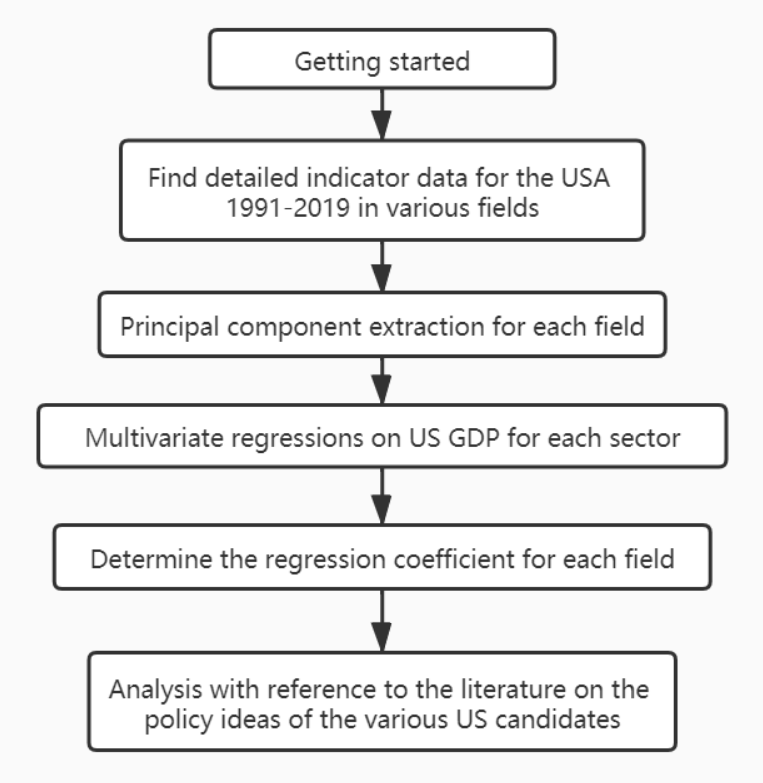
\includegraphics[width=0.7\linewidth]{screenshot001}
	\caption{Problem 1 Solving Process}
	\label{fig:screenshot001}
\end{figure}

\subsection{Model development and solving} %从原始数据中进行初步的特征提取
Different indicators are created to quantify the impact that the election of different candidates could have on the US economy.
In this problem, the key areas that influence the US economy are identified, a system of indicators that influence the US economy is established, and then relevant data is collected on these key areas of development, and principal component analysis is used to downscale the data for each area in turn, i.e. the principal components are derived. RStudio is used to develop multiple regression models of economic impact and then to collect data on the policies of the two candidates in different areas, which are then analysed using textual analysis of the relevant policies of the two candidates.

\subsubsection{Preparation of data}
In order to analyse the topic, we first need to look at the relevant data to determine the impact that the different candidates would have on the US economy if they took office in the 11 areas of economic development in the US: COVID19 infection rates, employment, transport, education, energy, agriculture, population, taxation, environmental protection, health care, banking and currency.

1. Collect relevant data for each of these areas (education as an example).

2. Construct a system of indicators that influence the development of education in the United States.
Based on the actual situation of the factors that influence the development of education, we have concluded 46 indicator variables that influence the development of education in the United States. 

They are shown in Figure 2 below.

\begin{figure}[H]
	\centering
	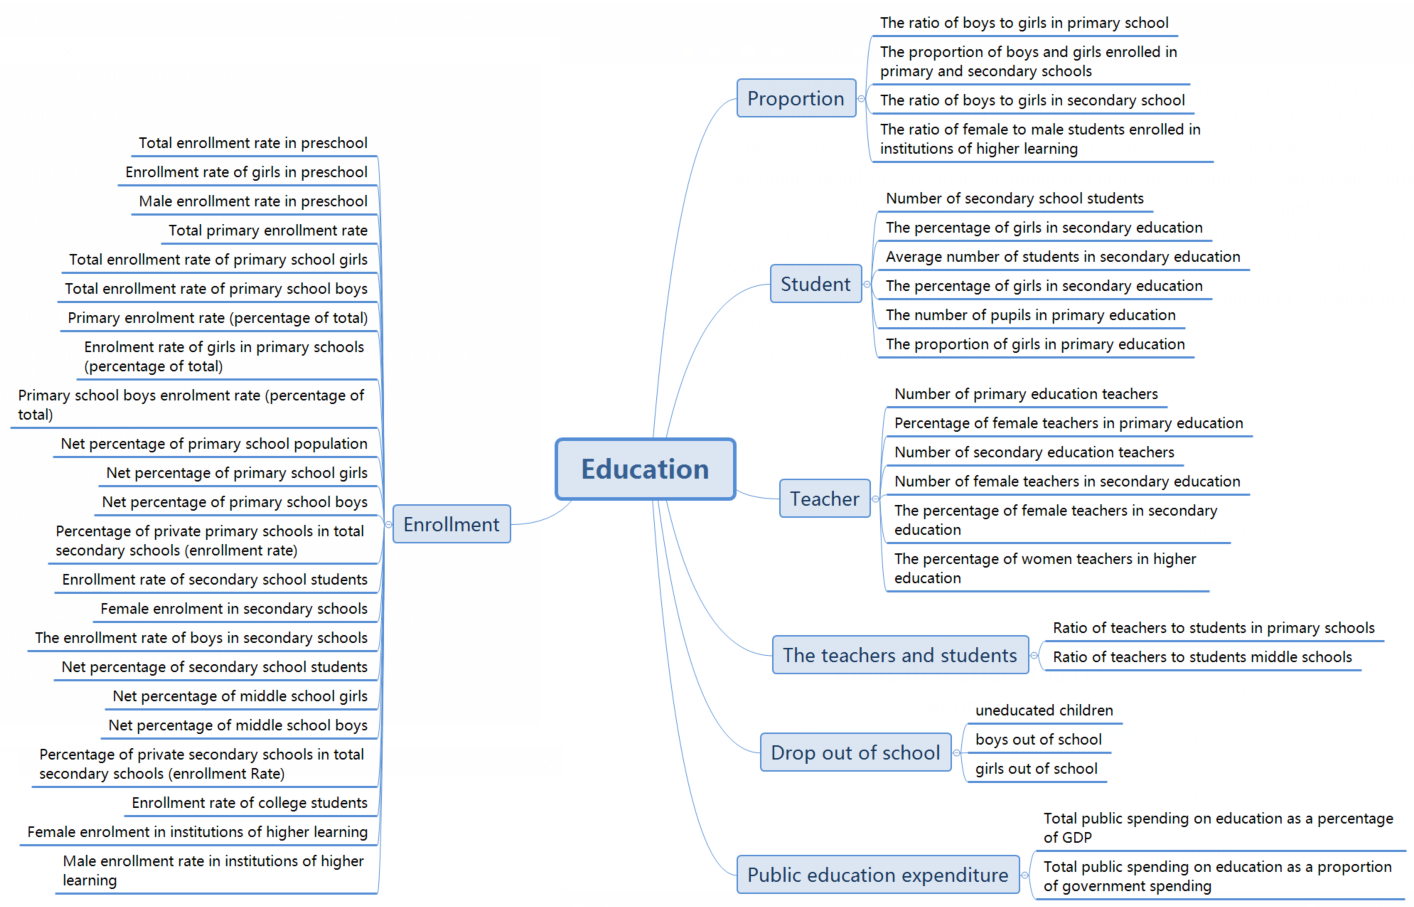
\includegraphics[width=\linewidth]{screenshot003}
	\caption{}
	\label{fig:screenshot003}
\end{figure}



\textbf{Take the education sector as an example}

According to Figure 1, there are 46 indicator variables for principal component analysis of education: 
\begin{lstlisting}
x_1,x_2,x_3,...,x_46, i.e., 
x_1={Secondary Education. Pupils}; 
x_2={Secondary education. Pupils}; 
x_3={Secondary Education. Students in general}; 
x_4={Secondary education. Percentage of girls}; 
x_5={Teacher-student ratio in secondary schools}; 
x_6={Enrolment . Secondary schools . Percentage of total}; 
x_7={Enrolment . Secondary schools . Female students . Percentage of total}; 
......
x_43={Gross enrolment ratio of boys in primary school. Net ratio}; 
x_44={out-of-school children. Primary school}; 
x_45={out-of-school girls . Primary schools}; 
x_46={out-of-school boys . Primary school}.
\end{lstlisting}

Specifying the number of principal components as 1 and using the education composite index to retain a large number of sub-information points in the sample, denoted as Y, gives.

\begin{equation}
Y=p_1x_1+p_2x_2+p_3x_3+p_4x_4+p_5x_5+…+p_{46}x_{46} 
\end{equation}
Of which, $ x_1,x_2,x_3,…,x_{46} $ are the variables for each indicator for the field of education in the USA and $ p_1,p_2,p_3,...,p_{46} $ are the principal component score coefficients for each indicator for the field of education in the USA.
Based on the data available on the development of the education sector in the USA from 1997-2019, the principal components of the education sector were extracted: (some data are shown in Table 1 below)
\begin{table}[H]
	\caption{Data on the US education sector 2000-2003}\label{tab:101} \centering
	\begin{tabular}{ccc}
		\toprule[1.5pt]
		Indicator Name        & 2018年    & 2019年      \\
		\midrule[1pt]
Secondary education, students                                              & 22593562 & 23087042 \\
Secondary education, students (\% of girls)                                & 48.99744 & 49.03448 \\
Secondary education, general students                                      & 22593562 & 23087042 \\
Secondary education, general students (\% of girls)                        & 48.99744 & 49.03448 \\
Teacher-pupil ratio in secondary schools                                   & 15.21729 & 15.15112 \\
School enrolment, secondary (\% of total)                                  & 92.3248  & 93.12471 \\
School enrolment, secondary, girls (\% of total)                           & 93.01242 & 93.87016 \\
School enrolment, secondary, boys (\% of total)                            & 91.67372 & 92.41859 \\
School enrolment, secondary (net \%)                                       & 85.31192 & 86.24302 \\
School enrolment, secondary, girls (net \%)                                & 86.5979  & 87.49322 \\
...&...&...\\
Gross enrolment ratio (net) of boys in primary school                      & 96.63585 & 96.27744 \\
Out-of-school children, primary school                                     & 826779   & 774457   \\
Out-of-school girls, primary school                                        & 402846   & 301354  \\
		\bottomrule[1.5pt]  
	\end{tabular}
\end{table}
\subsubsection{Principal components analysis}
Do a principal components analysis based on raw data relating to the development of the education sector in the USA from 1997-2019, specify the number of principal components as 1, call the package in R and run the program to obtain the score for the principal components (see Appendix 1 for code details), i.e. obtain the coefficients of the principal components score, as shown in Table 3 below.

\begin{table}[H]
	\caption{Coefficients for the principal component scores of the indicators in the field of education}\label{tab:102} \centering
	\begin{tabular}{cc}
		\toprule[1.5pt]
		Indicators & Principal component score \\
				\midrule[1pt]
		Secondary Education. Pupils                                                                                         & 0.83                      \\
		Secondary Education. Students .                                                     & -0.2                      \\
		Secondary education. Students in general& 0.82                      \\
		Secondary Education. General students & -0.2                      \\
		Teacher-student ratio in secondary schools& -0.77                     \\
		School enrolment. Secondary schools & 0.39                      \\
		School enrolment . Secondary schools& 0.26                      \\
		Enrolment... Secondary schools& 0.39                      \\
		Enrolment rates... Secondary schools& 0.41                      \\
		School enrolment... Secondary schools& 0.31                      \\
		School enrolment.... Secondary schools& 0.23                      \\
		School enrolment.... Secondary schools... Private& -0.84                     \\
		...&...\\
		Out-of-school children... Primary schools              & 0.86                      \\
		Girls out of school. Primary schools                                                                                & 0.81                      \\
		Out of School Boys. Primary school                                                                                  & 0.89 \\
		\bottomrule[1.5pt]                    
	\end{tabular}
\end{table}

Based on the above results, the equation for the principal components in the US education sector is derived as follows.
Equations for principal components in US education:
\begin{equation}
Y=p_1x_1+p_2x_2+p_3x_3+p_4x_4+p_5x_5+p_6x_6+p_7x_7+...+p_{45}x_{45}+p_{46}x_{46}
\end{equation}
where the coefficients are as shown above.

Calculate the education composite index based on the equation for principal components in the US education sector.
Based on the above equations, the US education composite index for 1997-2019 was calculated using Matlab programming (see Appendix 2 for code details), as shown in Table 4 below.

\begin{table}[H]
	\caption{US Education Composite Index 1997-2019}\label{tab:104} \centering
	\begin{tabular}{cc}
		\toprule[1.5pt]
		year & Education composite index \\
			\midrule[1pt]
		1997 & 46957349.65               \\
		1998 & 46224132.35               \\
		1999 & 44139353.25               \\
		2000 & 44331776.3                \\
		2001 & 47500826.12               \\
		2002 & 48700487.42               \\
		2003 & 48573758.39               \\
		2004 & 49511658.68               \\
		2005 & 49950828.02               \\
		2006 & 51273327.25               \\
		2007 & 51594879.88               \\
		2008 & 52402966.69               \\
		2009 & 53371759.9                \\
		2010 & 54720203.52               \\
		2011 & 55698979.55               \\
		2012 & 55714675.66               \\
		2013 & 55504249.83               \\
		2014 & 55493224.64               \\
		2015 & 55411783.33               \\
		2016 & 55755678.9                \\
		2017 & 55675617.55               \\
		2018 & 55922518.83               \\
		2019 & 55782254.68               \\
			\bottomrule[1.5pt]      
	\end{tabular}
\end{table}
\subsubsection{Standardised processing of data using z-score standardisation}
Data from the US Education Composite Index from 1997 to 2019 were standardised using z-score standardisation using the formula.

\begin{equation}
	X_{new}=\frac{X-\mu}{\sigma}=\frac{X-Mean(X)}{StdDev(X)}
\end{equation}
The z-score standardised and processed education composite index is shown in Table 5 below. 
\begin{table}[H]
	\caption{Standardised data for the US education composite index, 1991 to 2019}\label{tab:105} \centering
	\begin{tabular}{cc}
		\toprule[1.5pt]
		year & Education composite index \\
		\midrule[1pt]
		1991 & -1.595202495              \\
		1992 & -1.481259461              \\
		1993 & -1.367316425              \\
		1994 & -1.253373389              \\
		1995 & -1.139430355              \\
		1996 & -1.025487319              \\
		1997 & -0.626048618              \\
		1998 & -0.774172828              \\
		1999 & -1.195338911              \\
		2000 & -1.156465698              \\
		2001 & -0.51625576               \\
		2002 & -0.273900754              \\
		2003 & -0.299502493              \\
		2004 & -0.110028322              \\
		2005 & -0.021307541              \\
		2006 & 0.245863125               \\
		2007 & 0.310823034               \\
		2008 & 0.474072347               \\
		2009 & 0.669787491               \\
		2010 & 0.94219943                \\
		2011 & 1.139931298               \\
		2012 & 1.143102219              \\
		\bottomrule[1.5pt]      
	\end{tabular}
\end{table}

Using the same method of calculating the US Education Composite Index as described above, the other 10 areas of the US are calculated as follows
Standardised data for the composite indices, including standardised data for the transport network composite index, standardised data for the economic composite index, standardised data for the employment composite index, standardised data for the energy composite index, standardised data for the agricultural composite index, standardised data for the population composite index, standardised data for the tax composite index, standardised data for the environmental composite index, standardised data for the medical composite index and standardised data for the banking and currency composite index, see Appendix 3 - Appendix 13 for details of the composite indices for the above 10 areas. 
\begin{figure}[H]
	\centering
	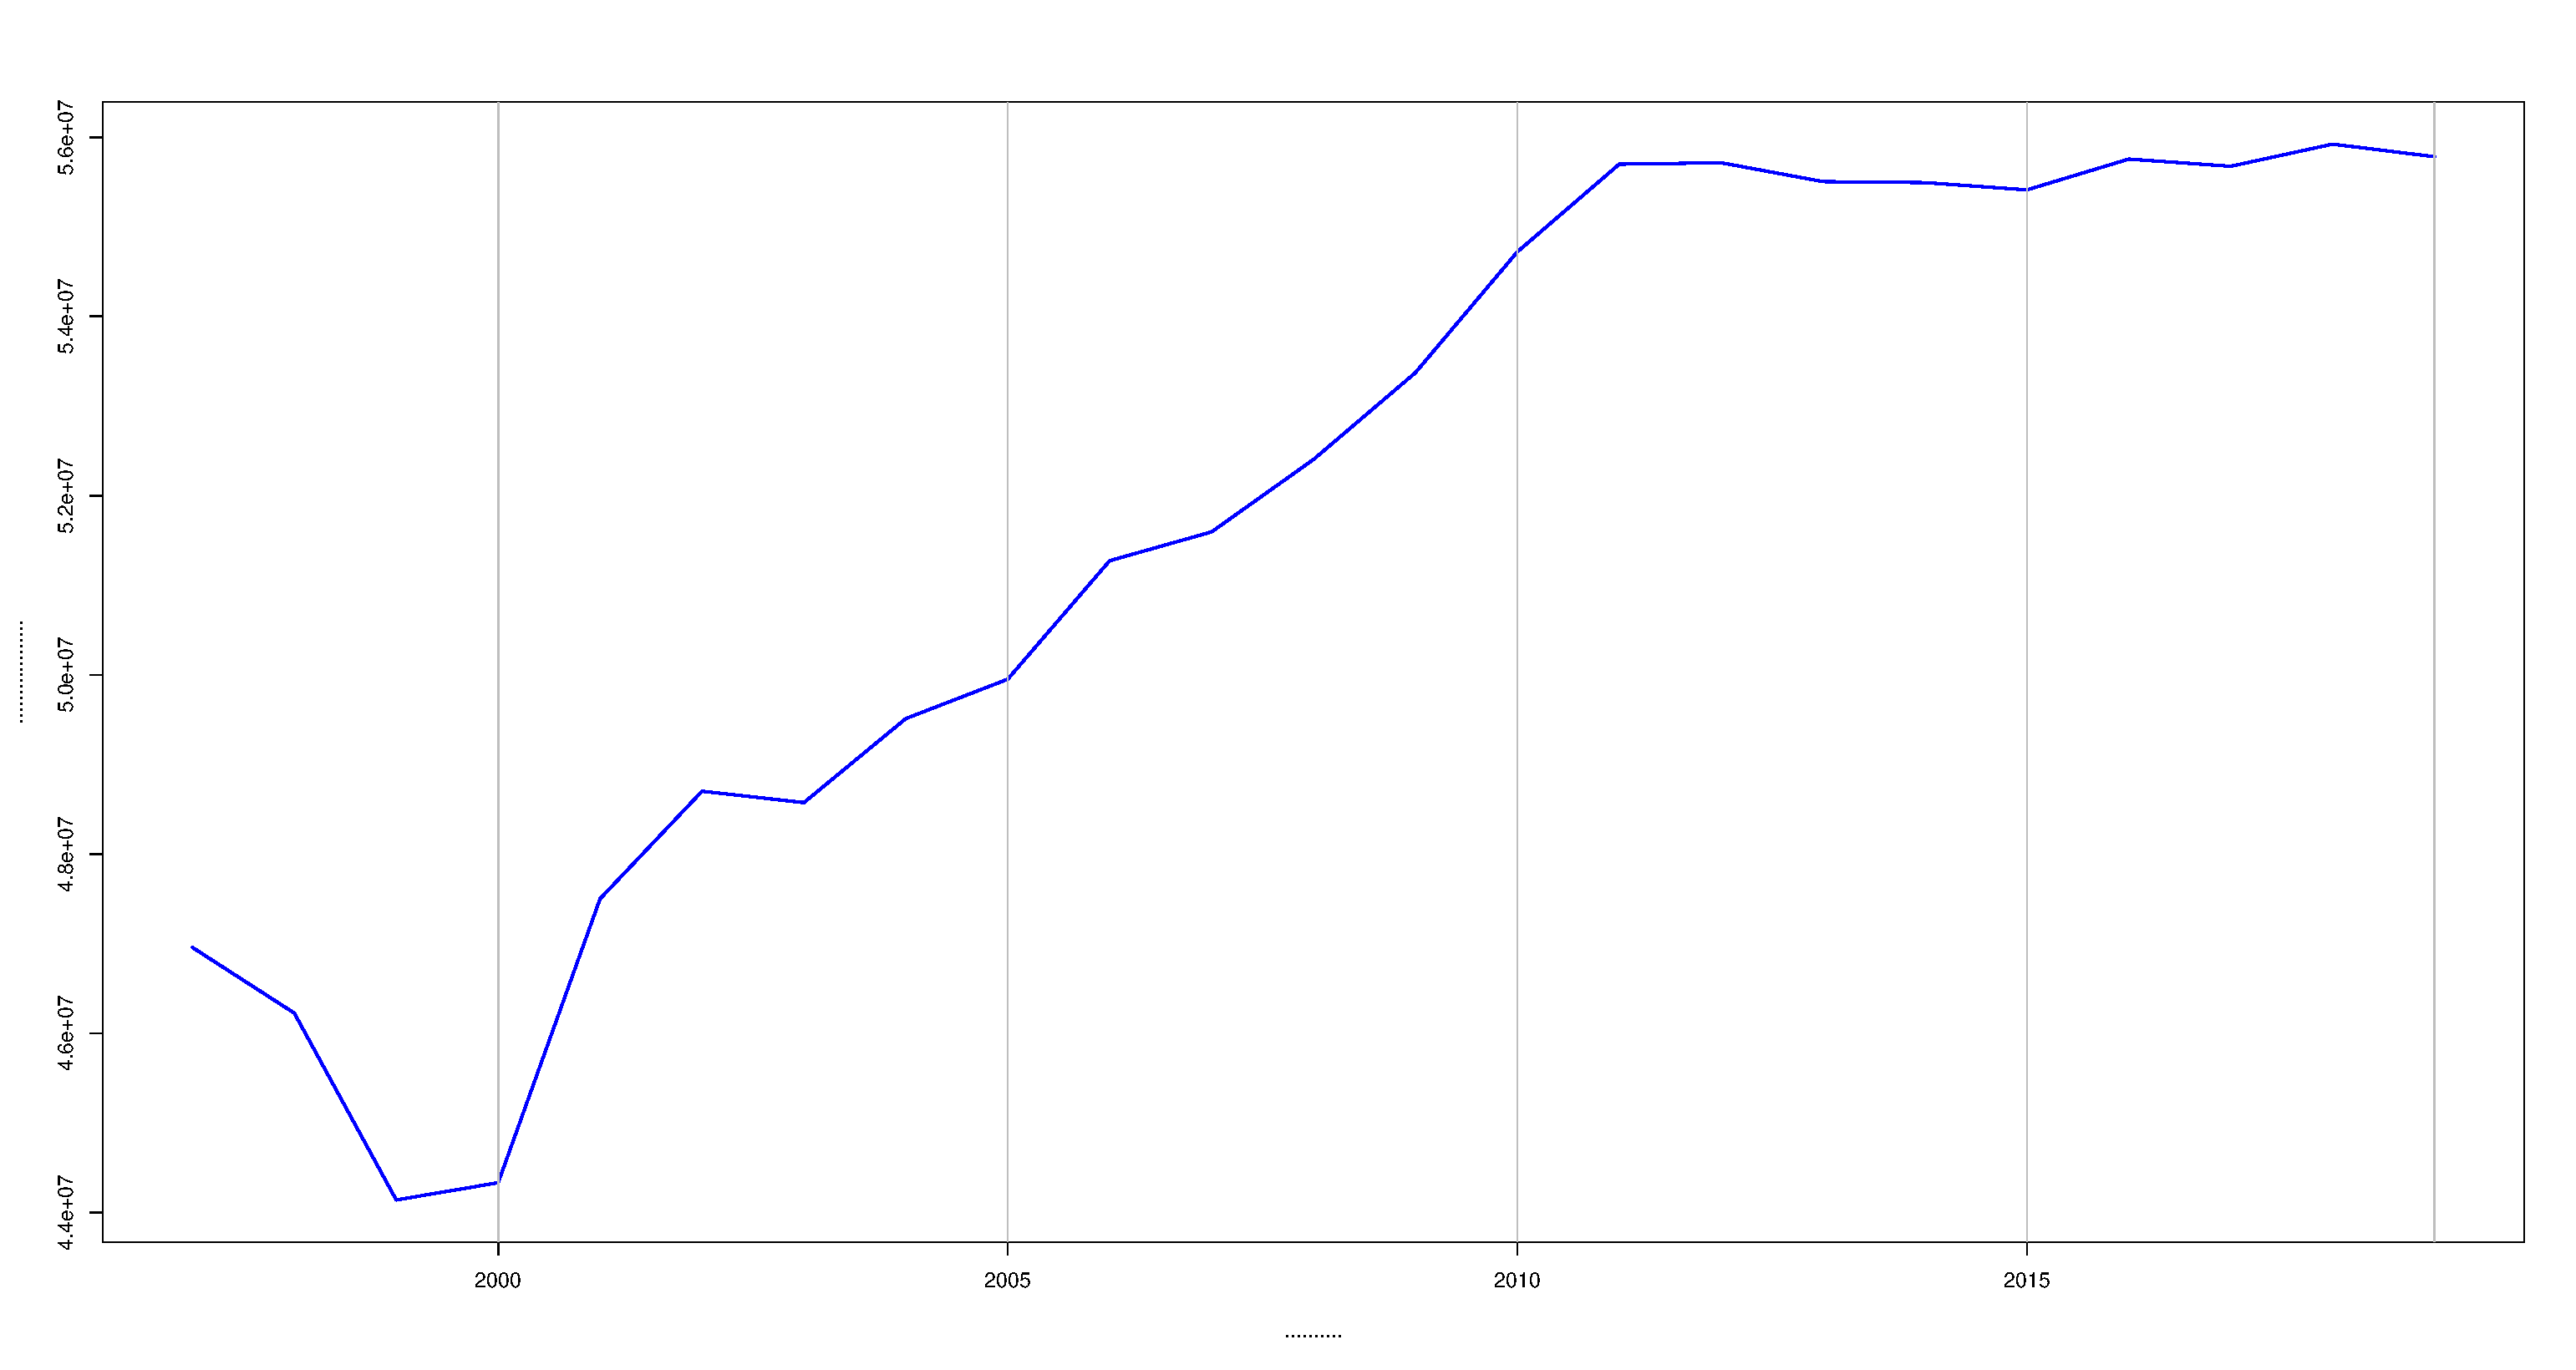
\includegraphics[width=\linewidth]{usa_edu}
	\caption{US Education Composite Index 1997-2019 Line Chart}
\end{figure}
\subsubsection{Modelling}
Defining a system of indicators to influence US economic development: Based on the data already prepared, a system of indicators to influence US economic development has been constructed by using as indicators for each of the 11 areas of COVID19 infection rates, employment, transport, education, energy, agriculture, population, taxation, environmental protection, health care and banking and currency, respectively, as a composite indicator, as shown in Figure 4 below.

\begin{figure}[H]
	\centering
	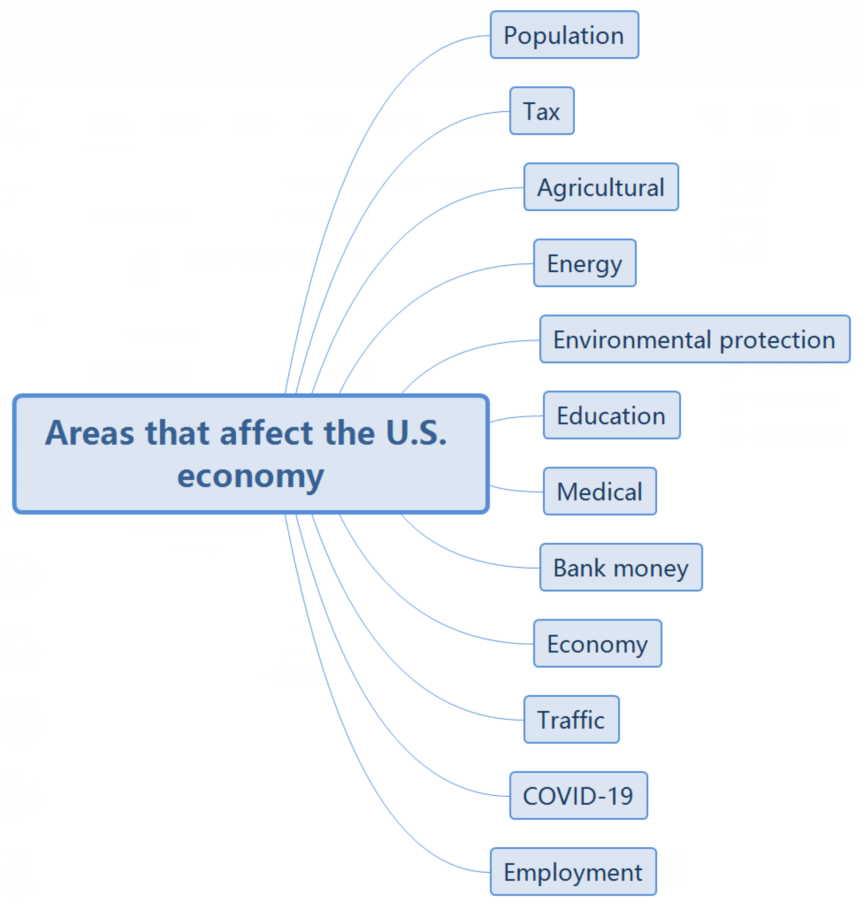
\includegraphics[width=0.65\linewidth]{screenshot005}
	\caption{A system of indicators affecting economic development in the US}
	\label{fig:screenshot005}
\end{figure}

According to Figure 4, there are 11 explanatory variables that affect economic development in the US: $ x_1,x_2,x_3,...,x_{11} $.

i.e.
\begin{lstlisting}
	x_1={standardised data from the Transportation Network Composite Index};
	x_2={standardised data from the Education Composite Index};
	x_3={standardised data from the Economic Composite Index};
	x_4={standardised data from the Employment Composite Index};
	x_5={standardised data for the energy composite index}; 
	x_6={standardised data for the agriculture composite index};
	x_7={standardised data for the population composite index}; 
	x_8={standardised data for the tax composite index}; 
	x_9={standardised data for the environmental composite index}
	x_10={standardised data for the medical composite index}
	x_11={standardised data for the bank currency composite index standardised data}. 
\end{lstlisting}

Also, the response variables: $ Y =\left\lbrace US\;GDP\right\rbrace  $. This yields 11 explanatory and response variables, which are predicted by a regression equation that determines the parameters of the explanatory variables. 
\begin{equation}
Y = \beta_0 + \beta_1x_1 + \beta_2x_2 + ...+ \beta_9x_9 + \beta_{10}x_{10} + \beta_{11}x_{11} + \epsilon_i
\end{equation}
where Y is the response variable: US Gross Domestic Product, $\beta $ is the regression coefficient and β is the parameter to be determined, $ \epsilon_i $ is the random error, $ x_1,x_2,x_3,...,x_{11} $ is the selected explanatory variable, i.e. the standardised data of the composite index of 11 areas influencing economic development in the US, $ \beta_1,\beta_2,\beta_3...,\beta_{11} $ is the regression coefficient for each influencing factor. 

In this paper, the R language is used, and the selected explanatory variables are all entered into a regression model, i.e. the parameters are estimated using the ordinary least squares method, which has the advantage of simplicity and speed of prediction. 

It is customary to consider the constant term as the coefficient of a dummy variable whose sample observation is always 1 during the parameter estimation process, so the number of explanatory variables for the model is 12. 

Expressed in matrix form, this would be:

$$ \textbf{Y}_{n\times 1}=\textbf{X}_{n\times(k+1)}\textbf{B}_{(k+1)\times 1}+\epsilon_{n\times 1}$$

$
\mathbf{X} = \left(
\begin{array}{cccc}
	1 & x_{11} & \ldots & x_{k1}\\
	1 & x_{12} & \ldots & x_{k2}\\
	\vdots & \vdots & \ddots & \vdots\\
	1 & x_{1n} & \ldots & x_{kn}\\
\end{array} \right)
$ , 
$
\mathbf{B} = \left(
\begin{array}{c}
	\beta_0 \\
	\beta_1\\
	\vdots \\
	\beta_k\\
\end{array} \right)
$ , $
\mathbf{Y} = \left(
\begin{array}{c}
	Y_1 \\
	Y_2\\
	\vdots \\
	Y_N\\
\end{array} \right)
$ , $
\mathbf{\epsilon} = \left(
\begin{array}{c}
	\epsilon_1 \\
	\epsilon_2\\
	\vdots \\
	\epsilon_n\\
\end{array} \right)
$ 

\hspace*{\fill}\\

where n=29 and k=11, satisfying $ n-k>=8 $; matrix Y represents the response variable, matrix X represents the design matrix, matrix B represents the vector of regression coefficients and matrix $ \epsilon $ represents the random error. 

Twenty-nine sets of sample observations were taken from the response and explanatory variables, as shown in Table 5 below.

\begin{figure}[H]
	\centering
	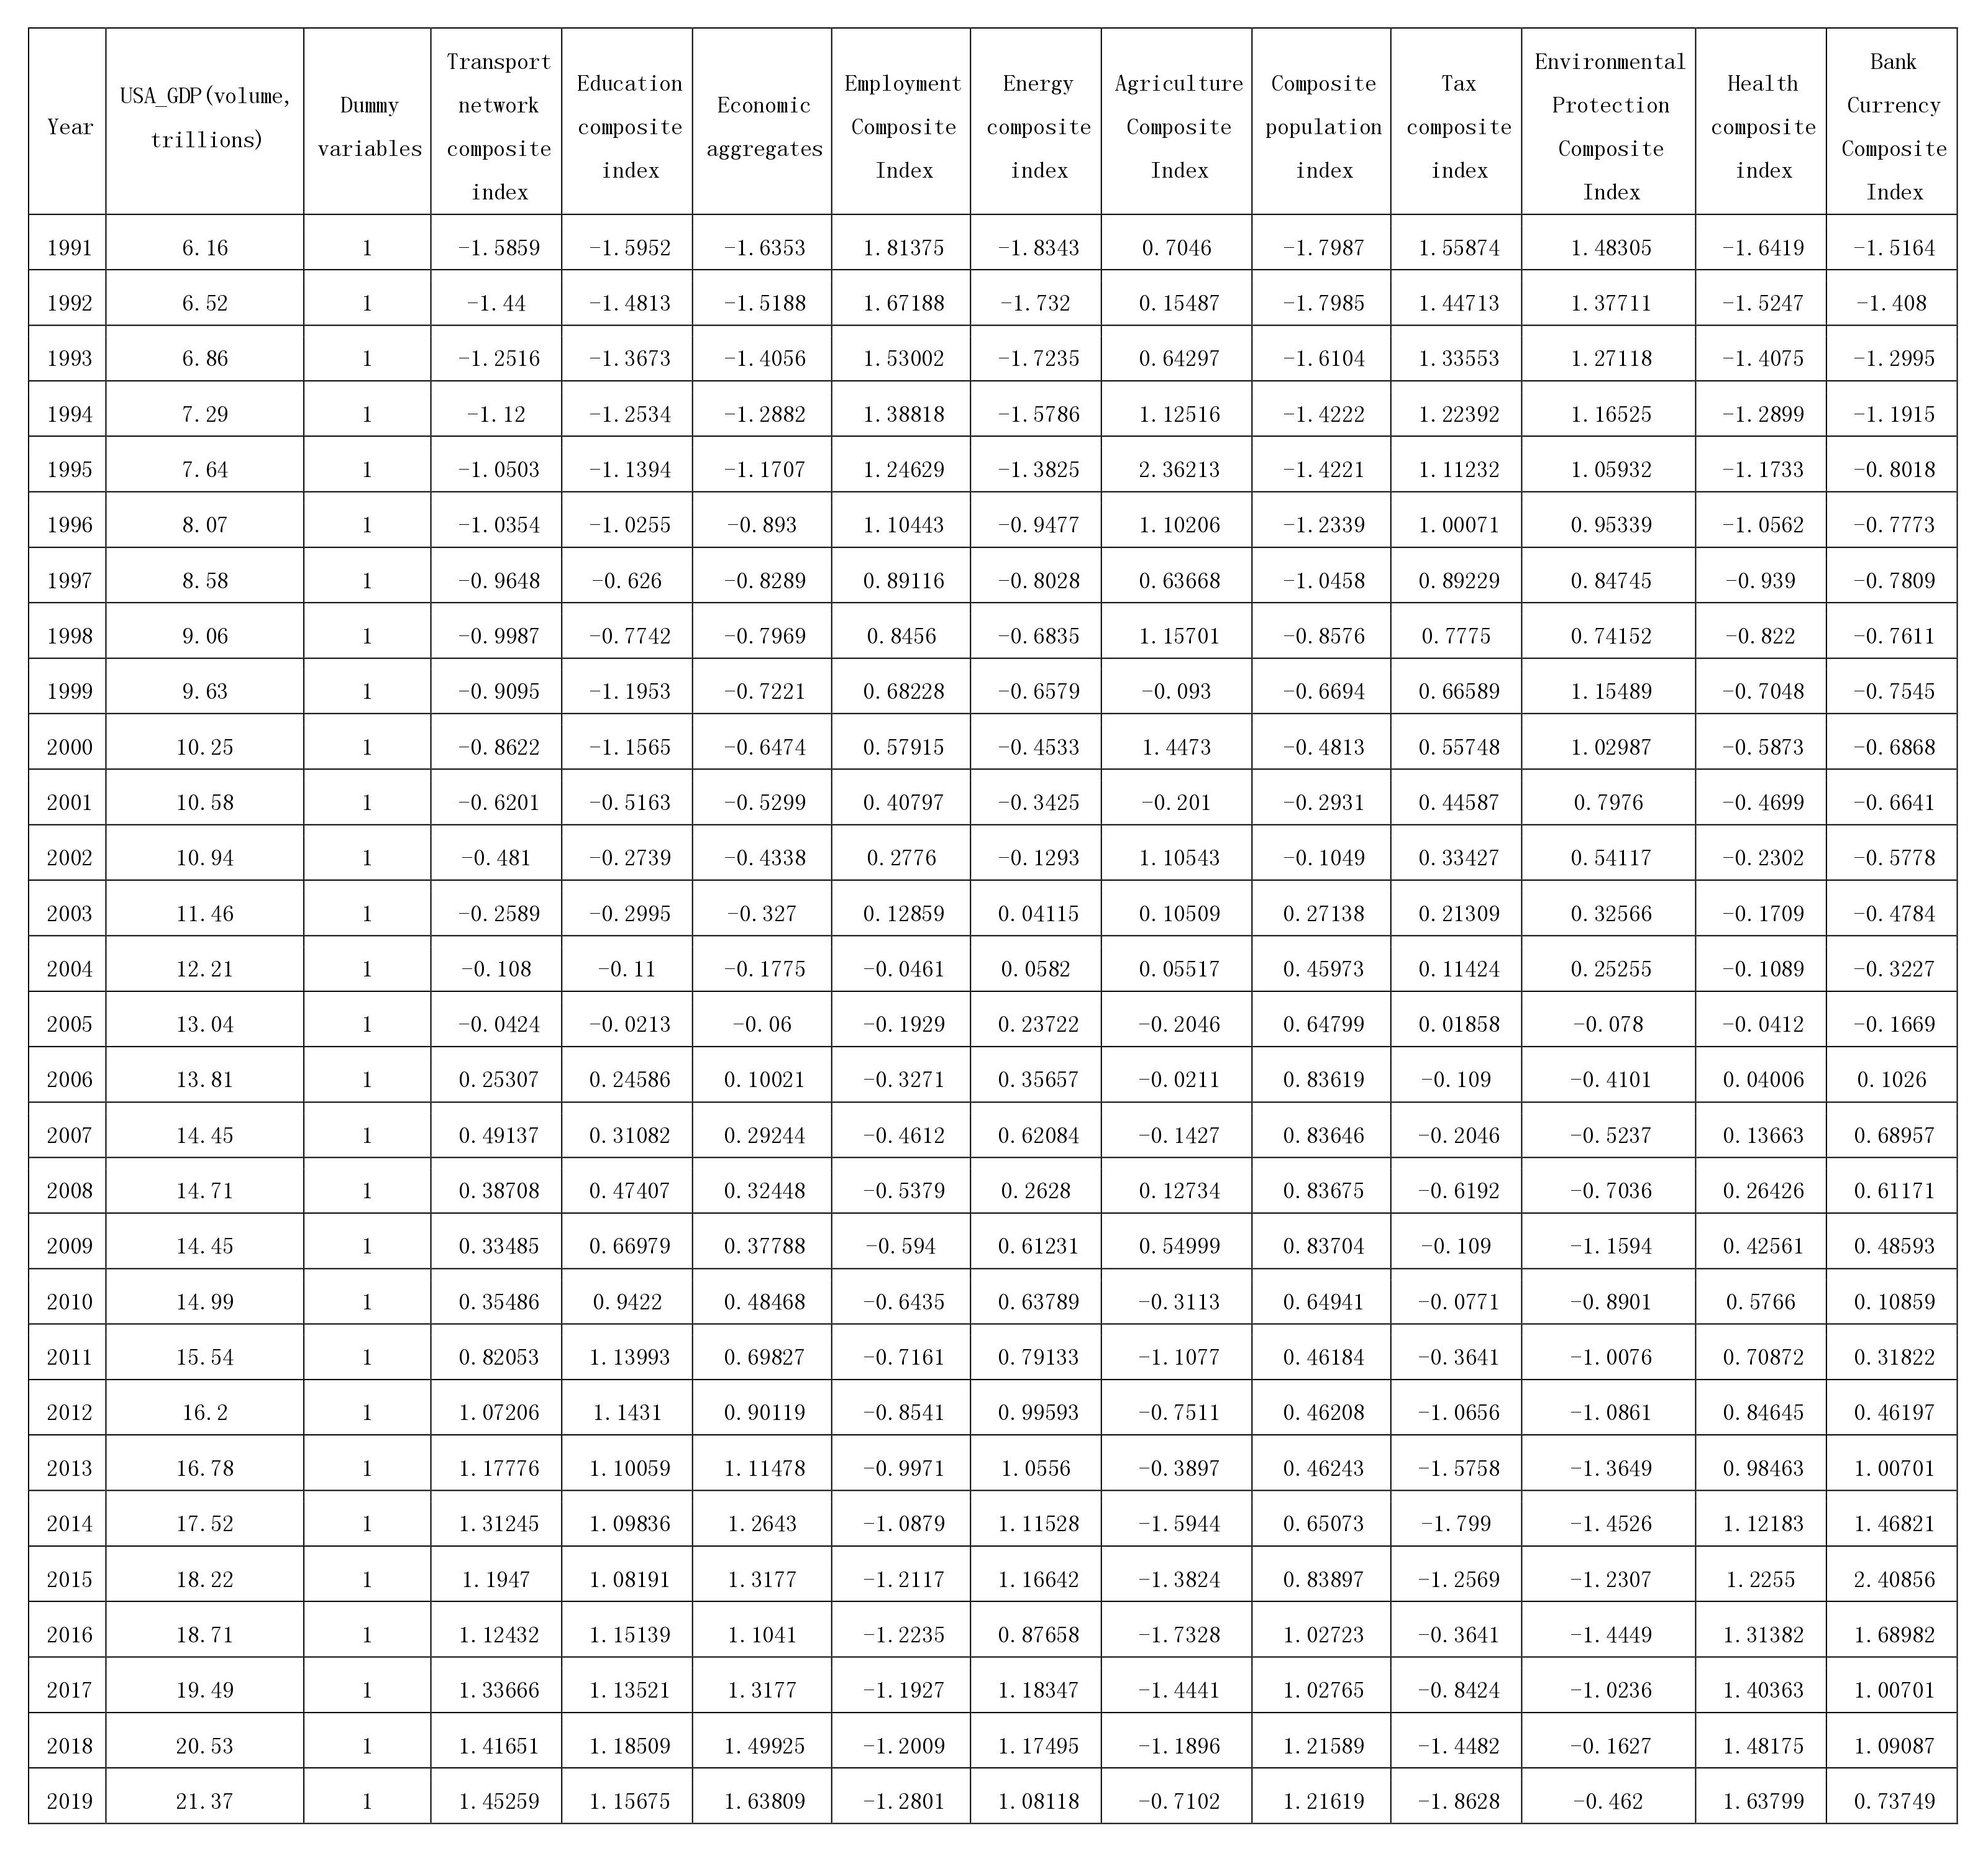
\includegraphics[width=\linewidth]{表5.jpeg}
	\caption{29 groups of sample observations}
\end{figure}

Expressions listing the parameter estimates:
\begin{equation}
\hat{Y} = \hat{\beta}_0 +\hat{\beta}_1x_1 +\hat{\beta}_2x_2 + \hat{\beta}_3x_3 +...+ \hat{\beta}_9x_9 +\hat{\beta}_{10}x_{10} +\hat{\beta}_{11}x_{11} 
\end{equation}

A set of equations for solving the parameter estimates according to the least squares principle:

\begin{equation}
	\left\{
	\begin{aligned}
		\frac{\delta}{\delta\hat{C}}Q & = & 0 \\
		\frac{\delta}{\delta\hat{\beta_1}}Q & = & 0 \\
		... & = & ...\\
		\frac{\delta}{\delta\hat{\beta_{11}}}Q & = & 0 \\
	\end{aligned}
	\right.
\end{equation}
其中,
\begin{equation}
\begin{aligned}
Q&=\sum_{n}^{i=1}e_i^2\\
&=\sum_{n}^{i=1}(Y_i-\hat{Y}_i)^2\\
&=\sum_{n}^{i=1}(Y_i-(\hat{\beta}_0 +\hat{\beta}_1x_1 +\hat{\beta}_2x_2 + \hat{\beta}_3x_3 +...+ \hat{\beta}_9x_9 +\hat{\beta}_{10}x_{10} +\hat{\beta}_{11}x_{11} ))^2
\end{aligned}
\end{equation}

Formal groups of equations are obtained for the estimated values of the parameters to be evaluated
\begin{figure}[H]
	\centering
	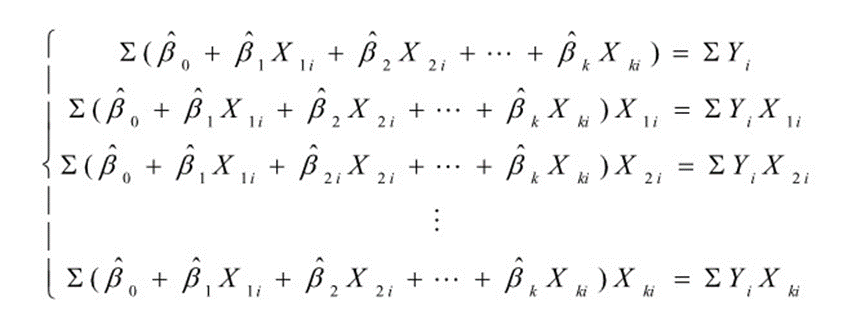
\includegraphics[width=\linewidth]{screenshot004}
	\caption{}
	\label{fig:screenshot004}
\end{figure}

Solving the linear algebraic set of these 12 equations gives an estimate of the 12 parameters to be evaluated

\begin{equation}
Q=\sum_{i=1}^{n}e_i^2=e'e=(Y-X\hat{\beta})'(Y-X\hat{\beta})
\end{equation}
Solve the set of partial derivative equations to obtain its least squares estimate:
\begin{equation}
\hat{\beta}=(X'X)^{-1}X'Y
\end{equation}
\subsubsection{Solving of models}

Solving the model for calculating the impact on economic development in the US: running the least squares procedure in R (see Appendix 14 for code details), which yields multiple regression results.

The model estimated the following results.
\begin{equation}
\begin{aligned}
\hat{Y}_t=12.93310+0.69428x_1-0.50169x_2+5.18329x_3+1.44506x_41.69210x_5 -0.05023x_6\\
+ 1.62642x_7+ 0.59604x_8+ 0.11109x_9+ 1.47196x_{10} -0.16434x_{11} 
\end{aligned}
\end{equation}
where the estimated values of the parameters to be evaluated are, respectively. 
\begin{equation}
	\begin{aligned}
		\hat{\beta}_0 = 12.93310 \\
		\hat{\beta}_1 = 0.69428\\
		\hat{\beta}_2= -0.50169\\
		\hat{\beta}_3= 5.18329\\
		\hat{\beta}_4= 1.44506\\
		\hat{\beta}_5 = -1.6921\\
		\hat{\beta}_6 = -0.05023\\
		\hat{\beta}_7= 1.62642\\
		\hat{\beta}_8= 0.59604\\
		\hat{\beta}_9= 0.11109\\
		\hat{\beta}_{10}=1.47196\\
		\hat{\beta}_{11}= -0.16434\\
	\end{aligned}
\end{equation}

\subsubsection{Possible impact on the US economy if different candidates are elected}
\begin{itemize}
	\item \textbf{(The likely impact of Donald Trump's election on the US economy)} 
\end{itemize}
The text tweeted by Republican candidate Donald Trump in recent years was selected for textual analysis (see Appendix 14 for code details), resulting in a tag cloud about Donald Trump, and the analysis of the tag cloud resulted in policy keywords that Donald Trump wanted to advocate, as shown in Figure 7 below.
\begin{figure}[H]
	\centering
	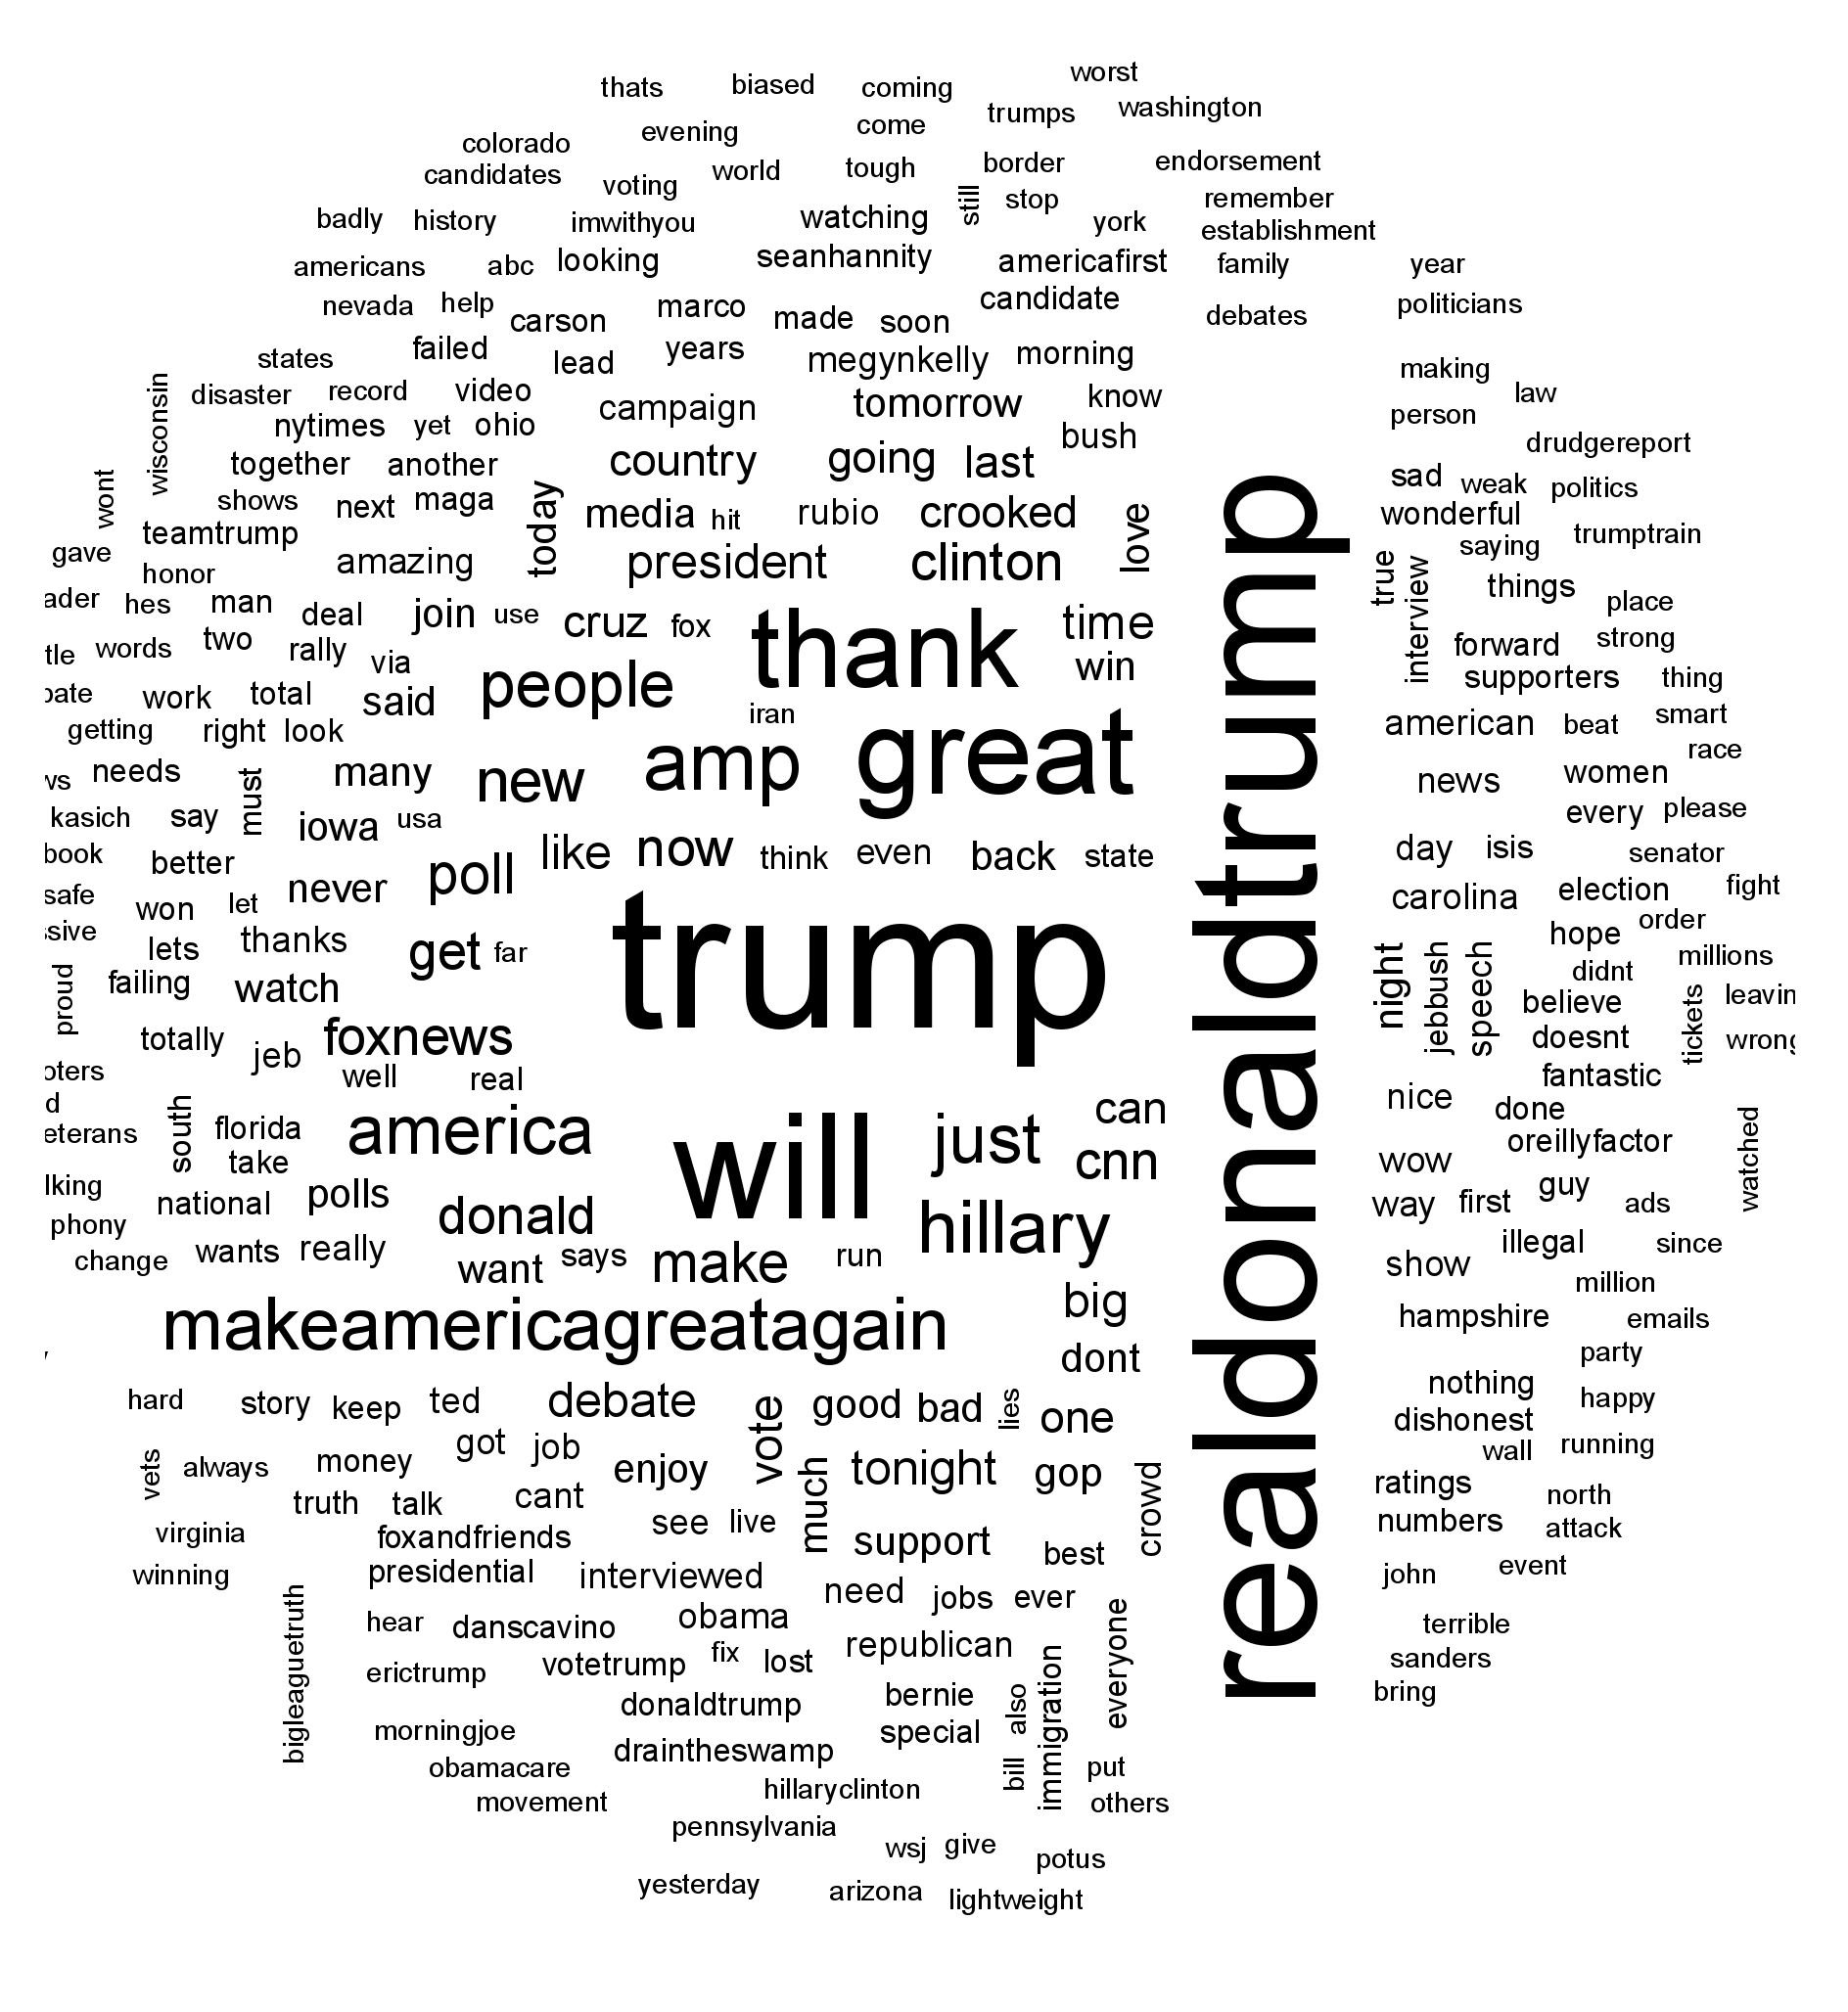
\includegraphics[width=\linewidth]{DT.jpeg}
	\caption{Donald Trump's tag cloud}
\end{figure}

In combination with a composite index of 11 areas of influence on the US economy and their corresponding estimates of the parameters to be estimated, specifically analysing the likely impact of the election of Donald Trump on the US economy, the explanatory and explanatory variables for the multiple regressions are shown in Table 6 below.
\begin{table}[H]
	\caption{Explanatory variables and their estimates}\label{tab:105} \centering
	\begin{tabular}{cc}
		\toprule[1.5pt]
	Explanatory variable & Parameter estimate \\
		\midrule[1pt]
		Transport            & 0.69428            \\
		Education            & -0.50169           \\
		Economic             & 5.18329            \\
		Employment           & 1.44506            \\
		Energy               & -1.6921            \\
		Agriculture          & -0.05023           \\
		population           & 1.62642            \\
		Tax                  & 1.59604            \\
		Environmental        & 0.11109            \\
		Health               & 1.47196            \\
		Bank                 & -0.16434          \\
		\bottomrule[1.5pt]      
	\end{tabular}
\end{table}

Table 6 above shows that the six explanatory variables that have a large impact on the response variable US GDP are: Economic Composite, Tax Composite, Energy Composite, Demographic Composite, Health Composite, Employment Composite, and the six explanatory variables that have a smaller impact are: Transportation Composite, Environmental Composite, Agriculture Composite, Banking and Currency Composite, and Education Composite.

Donald Trump's policies in the economic sphere: While his main focus is on boosting US economic growth and taking into account welfare requirements, his foreign-related economic policy mainly reflects a negative reaction to adjustment pressures arising from the evolution of the economy in an open environment. Possible impact on US economic development: His stimulus measures may help to boost US economic growth in the short term, but as his key ideas are on the opposite side of the law, it is difficult to significantly increase the US economic growth rate in the long term.

Donald Trump's policy ideas in the area of taxation: In terms of reforming personal income tax, Trump proposes to change the 7-tier cumulative tax rate on ordinary income to 3 tiers: 10\%, 25\% and 35\%. Trump plans to abolish the current minimum tax levels, which would reduce the tax burden on higher income earners. In response to the "deduction issue", Trump proposes to double the standard deduction (current: \$6,300 for individuals, \$12,600 for couples) and to abolish most deductions, leaving only two: the Section 170 charitable deduction and the Section 163 primary deduction. Housing loan interest deduction. Potential impact on US economic development: Trump's personal income tax reform could simplify the current tax system, but only the highest income earners will benefit the most. The pass-through entity tax reform, while cutting taxes for high-income earners, may lead to aggressive tax avoidance by high-income earners and will not benefit low and middle-income earners.

Donald Trump's policy ideas in the agricultural sector: to keep agriculture afloat. The Trump administration has added agricultural trade assistance programmes to the existing forms of agricultural subsidies, which include market promotion programmes, food procurement and distribution programmes and agricultural trade promotion programmes. Potential impact on US economic development: Leading to violations of WTO rules, these aid programmes stabilise agricultural production while also distorting markets. The US is likely to exceed its 'yellow box' cap on agricultural subsidies in 2019 as part of its WTO commitments.

Donald Trump's policy ideas in the area of immigration: emphasis on the use of executive power to implement monist immigration policy reforms that prioritise national sovereignty and roll back market and human rights. Potential impact on US economic development: This has had a ripple effect in US domestic politics and at the level of international relations. In the case of US domestic politics, this has had a negative impact on community relations, economic development and the political ecology, but has helped to strengthen Trump's voter base.
\begin{itemize}
\item \textbf{(The likely impact of Joe Biden's election on the US economy)}
\end{itemize}
Texts tweeted by Democratic Party candidate Joe Biden in recent years were selected for textual analysis (see appendix 14 for code details) to create a tag cloud on Joe Biden, and the analysis of the tag cloud led to the policy keywords Joe Biden wanted to advocate, as shown in figure 9 below.

\begin{figure}[H]
	\centering
	
\includegraphics[width=0.9\linewidth]{BT.jpeg}
	\caption{Joe Biden's tag cloud}
\end{figure}

Overall, the US economy is seen as a mixed bag since the election of Joe Biden, and the recovery process may continue to be a "pain and gain" concerto.

Joe Biden's policy ideas on the economic front: greater fiscal stimulus for Trump, a greater focus on green energy spending, and tax increases on high-income brackets and technology companies. The combination with a divided Congress will make the size of his fiscal stimulus likely to be smaller than the amount advocated in his campaign, and a small new round of fiscal stimulus is still likely to be landed. Possible impact on US economic development: some degree of economic stimulus, but less of a boost to employment and inflation, which is less sustainable as it is biased towards short-term cash flows and the subsequent multiplier effect is relatively small.

\subsection{Model testing}

Check for correlations between variables:
\begin{figure}[H]
	\centering
	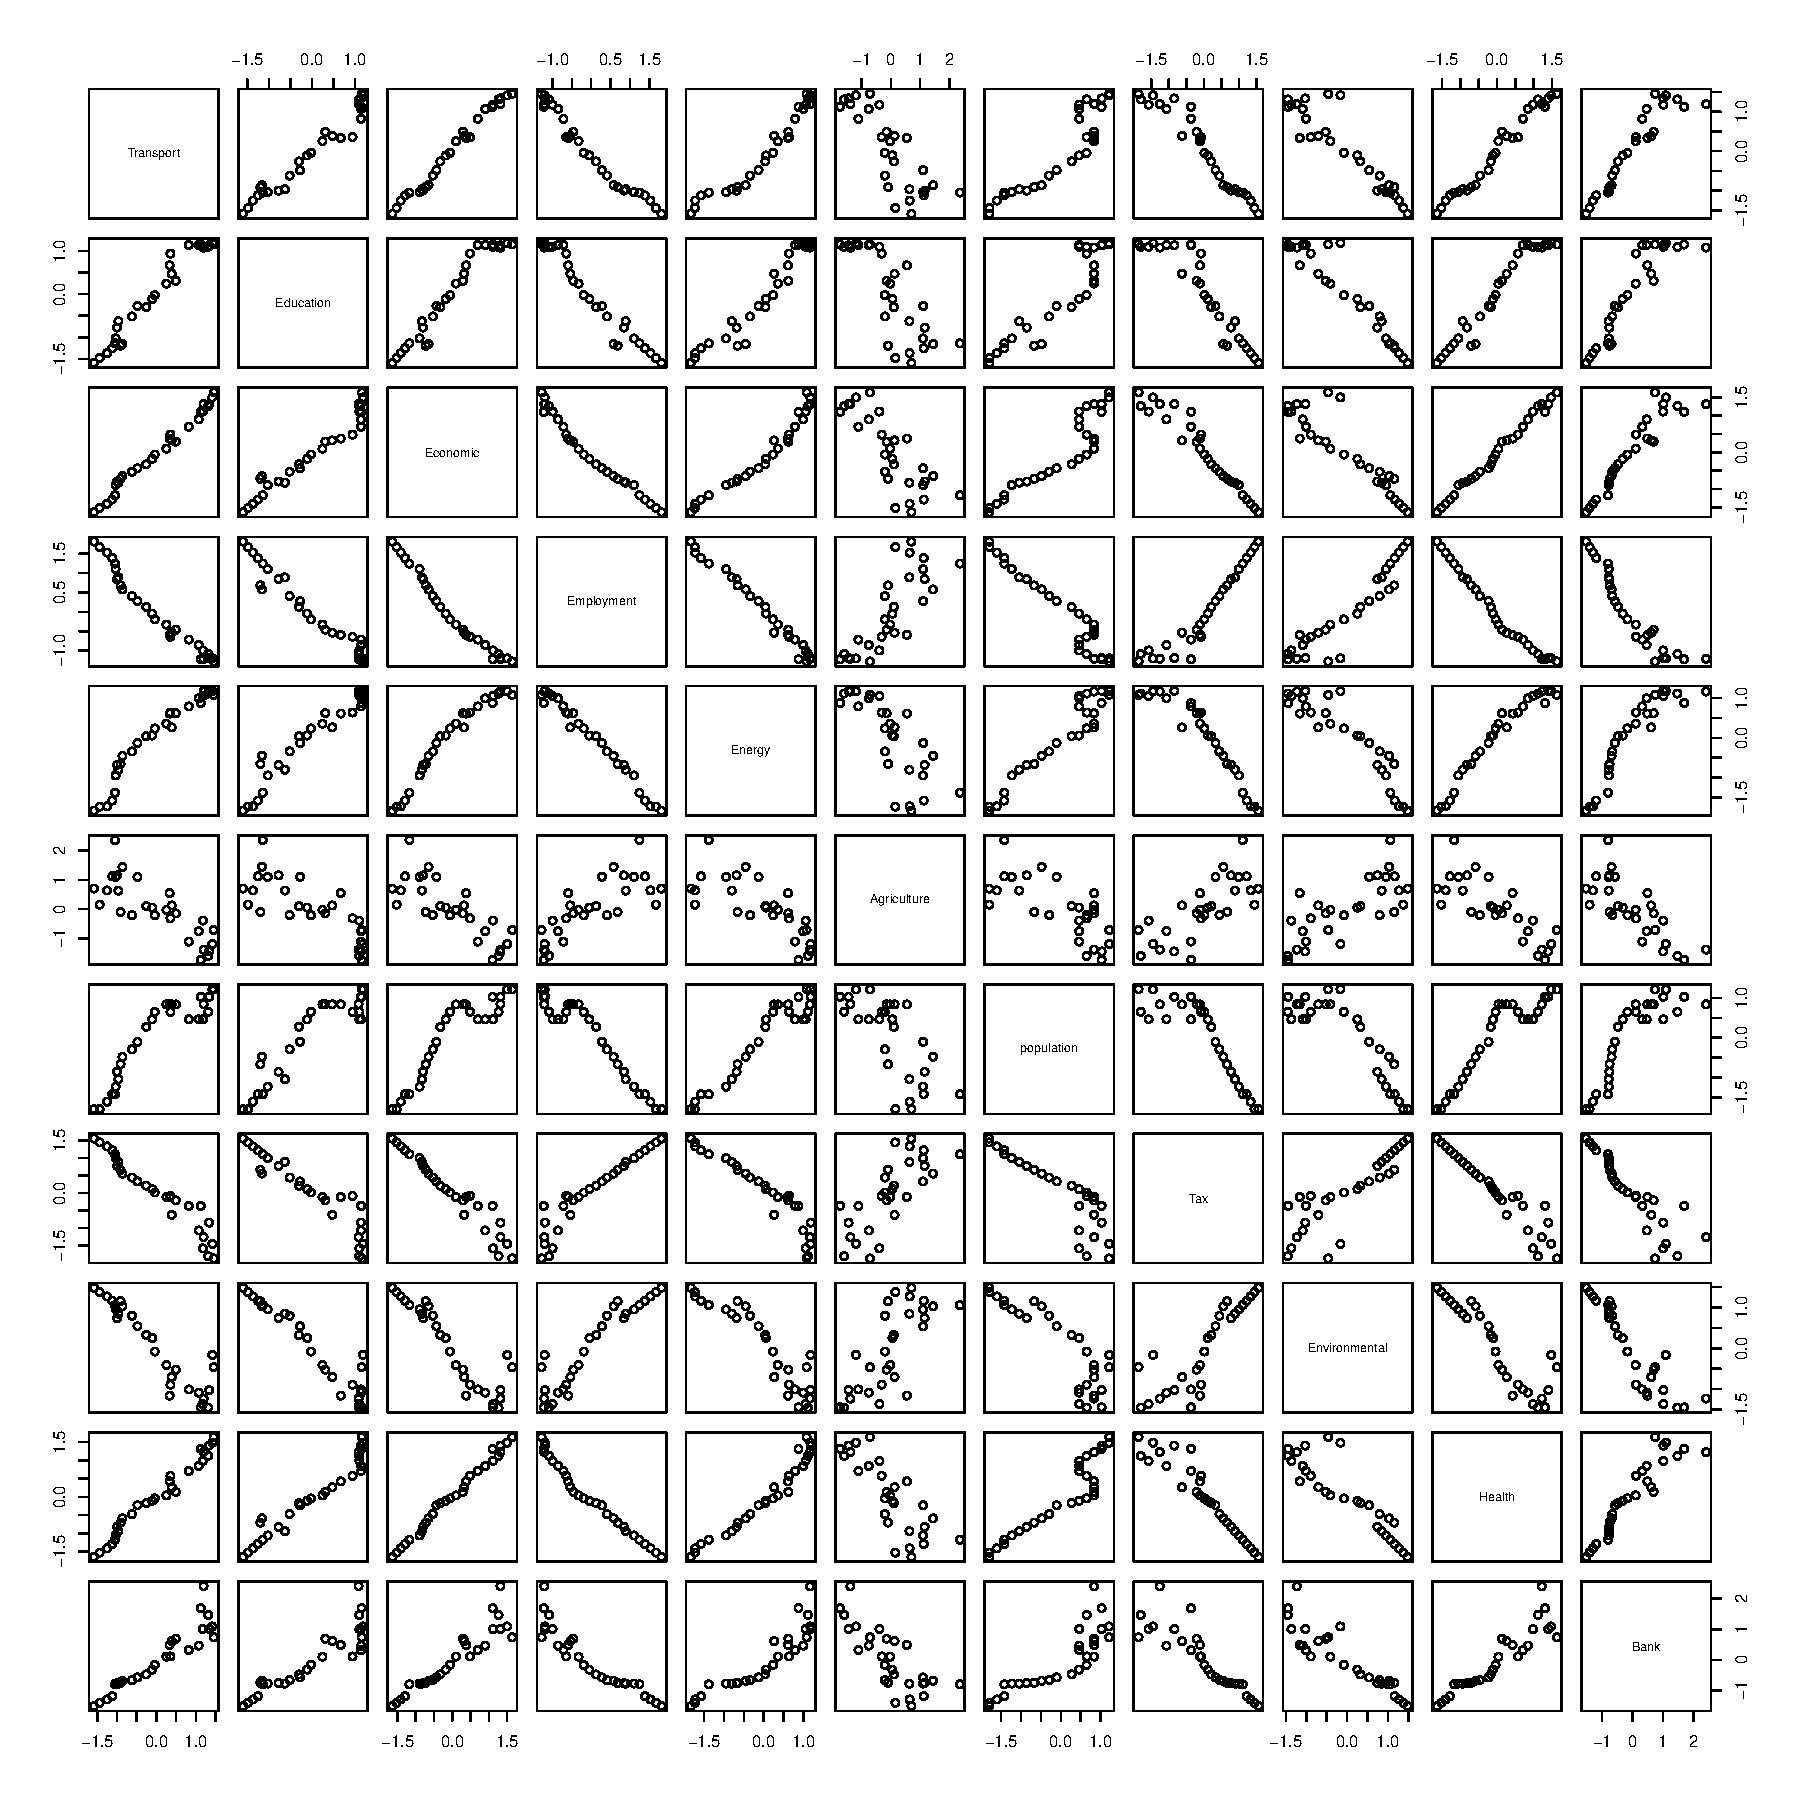
\includegraphics[width=\linewidth]{cor}
	\caption{correlations between variables}
\end{figure}

The corresponding Estimate, Std. Error, t value and Pr(>|t|) for the parameters to be evaluated are shown below. 
\begin{lstlisting}[language=r]
Residuals:
Min       1Q   Median       3Q      Max 
-0.44285 -0.13036  0.04252  0.09040  0.31347 

Coefficients:
              Estimate Std. Error t value Pr(>|t|)    
(Intercept)   12.93310    0.04539 284.918  < 2e-16 ***
Transport      0.69428    0.48961   1.418 0.174253    
Education     -0.50169    0.36823  -1.362 0.190842    
Economic       5.18329    0.95159   5.447 4.35e-05 ***
Employment     1.44506    1.23417   1.171 0.257800    
Energy        -1.69210    0.41537  -4.074 0.000790 ***
Agriculture   -0.05023    0.08479  -0.592 0.561410    
population     1.62642    0.34519   4.712 0.000201 ***
Tax            0.59604    0.24060   2.477 0.024036 *  
Environmental  0.11109    0.26439   0.420 0.679605    
Health         1.47196    0.75640   1.946 0.068377 .  
Bank          -0.16434    0.19197  -0.856 0.403851    
---
Signif. codes:  0 ‘***’ 0.001 ‘**’ 0.01 ‘*’ 0.05 ‘.’ 0.1 ‘ ’ 1

Residual standard error: 0.2444 on 17 degrees of freedom
Multiple R-squared:  0.9982,	Adjusted R-squared:  0.9971 
F-statistic: 867.1 on 11 and 17 DF,  p-value: < 2.2e-16
\end{lstlisting}

In the Pr(>|t|) column, you can see that the regression coefficients are significantly non-zero, indicating that for every change in each area, GDP would be expected to increase or decrease.

The R-squared term shows that the model can explain 99.82\% of the variance in body weight, which is also the sum of the actual and predicted values.

The standard error of the residuals is considered to be the average error of the model in predicting GDP using the principal components of each domain. F-statistics
The quantity tests whether all the predictor variables predict response variables above a certain probability level.

\subsubsection{Regression diagnosis}
\begin{lstlisting}[language=r]
> confint(ins_model)
                   2.5 %     97.5 %
(Intercept)   12.8373336 13.0288729
Transport     -0.3387061  1.7272661
Education     -1.2785997  0.2752149
Economic       3.1756110  7.1909611
Employment    -1.1588123  4.0489398
Energy        -2.5684494 -0.8157504
Agriculture   -0.2291266  0.1286709
population     0.8981248  2.3547166
Tax            0.0884219  1.1036554
Environmental -0.4467115  0.6688995
Health        -0.1239006  3.0678281
Bank          -0.5693537  0.2406715     
\end{lstlisting}

For example, if Economy changes by 1\%, GDP will change within the 95\% confidence interval [3.1756110,7.1909611]; since the confidence interval for Transport contains 0, it can be concluded that the change in Transport is independent of GDP when all other variables are unchanged. 
However, your belief in these results is based on the premise that your data meet the statistical assumptions.

\begin{figure}[H]
	\centering
	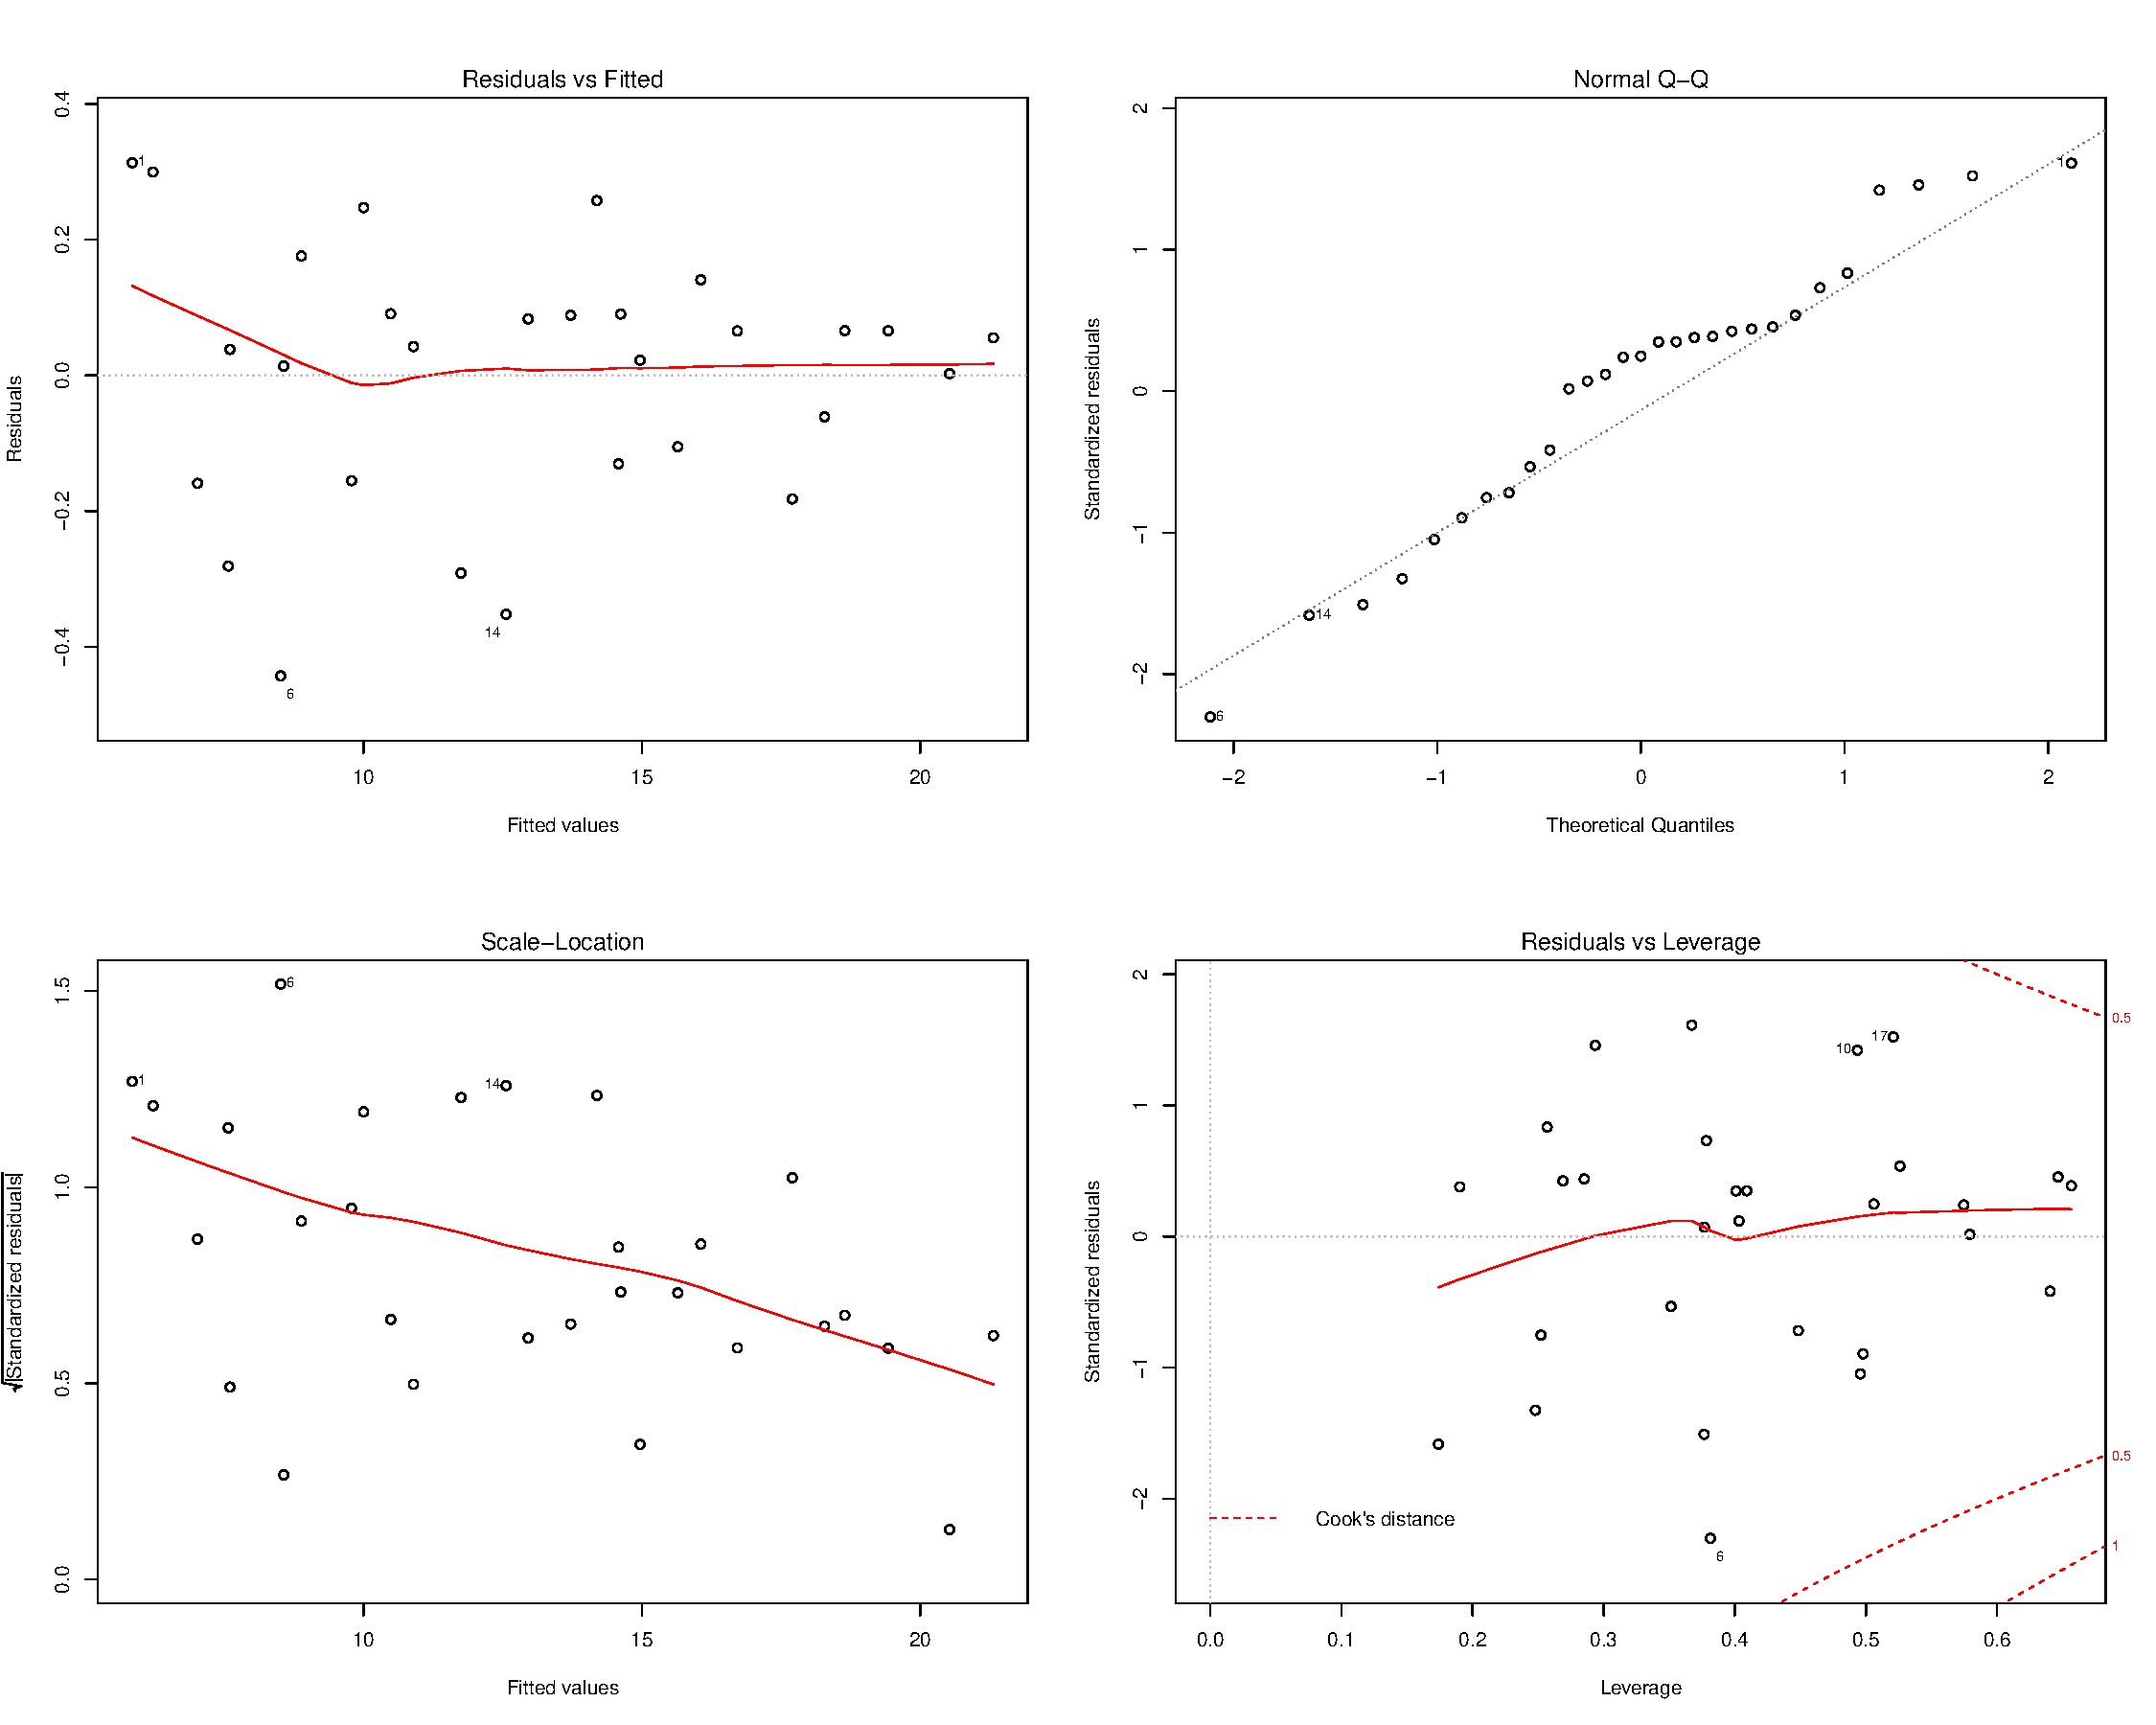
\includegraphics[width=0.7\linewidth]{四幅图}
	\caption{Four graphs to evaluate the fit of the model}
\end{figure}

This second set of plots shows a good polynomial regression fit, which conforms to the assumptions of linearity, residual normality (except for observation 13) and homoskedasticity (constant residual variance).
%%%%%%%%%%%%%%%%%%%%%%%%%%%%%%%%%%%%%%%%%%%%%%%%%%%%%%%%%%%%%

\section{Model Establishment and Solution of Problem 2}
A model based on indicators to quantify the likely impact of the election of different candidates on the Chinese economy
In the second question, we choose the standardised composite index of each sector as the independent variable and China's GDP as the dependent variable, establish a multiple regression model based on principal component analysis, obtain the weights of each index that affects China's GDP, and predict the impact on China's economy after the election of the two candidates through textual analysis of their policies.

\subsection{Development and solution of multiple regression models}

\subsubsection{Identify explanatory and response variables for the model.}
n the first question, we clarified that the extent to which each US sector affects the US economy differs, and similarly, the policies of the two candidates after their election affect China differently by influencing the development of each US sector. We therefore use the standardised data of the US composite index for each sector as explanatory variables for our model, i.e. we assume that 
\begin{lstlisting}
x1={standardised model of the transportation network composite index}; 
x2={standardised data of the education composite index};
x3={standardised data of the economic composite index};
x4={standardised data of the employment composite index};
x5={standardised data of the energy composite index};
x6={standardised data of the agricultural composite index}; 
x7={standardised data of the energy composite index index standardised data}; 
x8={standardised data for the tax composite index}; x9={standardised data for the environmental composite index}; 
x10={standardised data for the medical composite index}; x11={standardised data for the bank currency composite index}.
\end{lstlisting}

Also assume the model response variable: $ Y=\left\lbrace China's GDP (gross domestic product)\right\rbrace . $
\subsubsection{Modelling}
In order to find the relationship between the explanatory and response variables, we assume that the 11 explanatory variables have a multicollinear relationship with the response variables and that the prediction of the response variables is achieved by determining the parameters of the 11 explanatory variables.

\begin{equation}
	Y = \beta_0 + \beta_1x_1 + \beta_2x_2 + ...+ \beta_9x_9 + \beta_{10}x_{10} + \beta_{11}x_{11} + \epsilon_i
\end{equation}
where Y is the response variable: US Gross Domestic Product, $\beta $ is the regression coefficient and β is the parameter to be determined, $ \epsilon_i $ is the random error, $ x_1,x_2,x_3,...,x_{11} $ is the selected explanatory variable, i.e. the standardised data of the composite index of 11 areas influencing economic development in the US, $ \beta_1,\beta_2,\beta_3...,\beta_{11} $ is the regression coefficient for each influencing factor. 

The number of explanatory variables for this model is also 12 because they are the same as the explanatory variables used in the first question. 29 sample observations are taken from both variables, depending on the relationship between the response and explanatory variables.

According to the Least Squares Theorem, the equations are listed and solved to give an estimate of the 12 parameters to be evaluated.

Expressions for parameter estimates based on 29 sample sets of observations from multiple regression models affecting China's economic development.
\begin{equation}
	\hat{Y} = \hat{\beta}_0 +\hat{\beta}_1x_1 +\hat{\beta}_2x_2 + \hat{\beta}_3x_3 +...+ \hat{\beta}_9x_9 +\hat{\beta}_{10}x_{10} +\hat{\beta}_{11}x_{11} 
\end{equation}

\subsubsection{Solving of models}
Solve the model that calculates the impact on China's economic development.
Running the program in R using the least squares method (see Appendix 14 for code details) yields multiple regression results. 

The model estimated the following results.

\begin{equation}
	\begin{aligned}
		\hat{Y}_t= 4.74032+ 0.68066x_1- 0.03972x_2+ 5.75766x_3+2.38472x_4- 2.64365x_5\\
		- 0.20557x_6+ 0.24214x_7+ 6.9742x_{8}- 0.40180x_{9}+ 0.55964x_{10}- 0.21679x_{11}
	\end{aligned}
\end{equation}

\subsubsection{Possible impact on the US economy if different candidates are elected}

The estimates of the explanatory variables for the multiple regressions are shown in the table below, by combining a composite index of the 11 areas affecting economic development in the US with estimates of their corresponding parameters to be estimated.
\begin{table}[H]
	\caption{Explanatory variables and their estimates}\label{tab:105} \centering
	\begin{tabular}{cc}
		\toprule[1.5pt]
		Explanatory variable & Parameter estimate \\
		\midrule[1pt]
		Transport            & 0.68066            \\
		Education            & -0.03972           \\
		Economic             & 5.75766            \\
		Employment           & 2.38472            \\
		Energy               & -2.64365           \\
		Agriculture          & -0.20557           \\
		population           & 0.24214            \\
		Tax                  & 6.9742             \\
		Environmental        & -0.4018            \\
		Health               & 0.55596            \\
		Bank                 & 4.21679           \\
		\bottomrule[1.5pt]      
	\end{tabular}
\end{table}

From the table above, the six explanatory variables that have a large impact on the response variable Chinese GDP are: taxation composite, economic composite, bank and currency composite, energy composite, employment composite and transport composite; the six explanatory variables that have a smaller impact are: education composite, agriculture composite, population composite, environmental composite, health composite and transport composite.
\begin{itemize}
	\item \textbf{(The likely impact of Donald Trump's election on the China economy)} 
\end{itemize}

Consistent with the text analysed in Question 1, we can derive one policy keyword that Donald Trump wants to advocate - making America great again - and from the keyword and related literature we can conclude that.

Donald Trump's policy ideas in the area of banking and monetary policy: tight monetary policy and quantitative easing, which has led to a large inflow of industrial capital into the United States, has both advantages and disadvantages for China and has more negative effects, mainly on China's inflation and economic growth rate, which will have a more negative impact.

Donald Trump's policy ideas in the area of banking and currency: tax reform, China's need to guard against the elimination of interest on borrowing and outright tax rebates on services, etc. in the tax reform and the "going out" of Chinese companies by taking steps to reduce the tax burden on US companies.

Donald Trump's policy proposition in the field of population: the immigration policy, on the one hand, will have a certain negative impact on the cooperation between Chinese and American talents and academic exchanges, and on the other hand, it will provide opportunities for the global flow of talents to China, providing opportunities for China to attract more overseas talents.

Donald Trump's policies in the economic sphere: revitalising the importance of the US economy while curbing the rapid development of China's economy and technology will, in the case of China, curb the development of China's high-tech industry and hinder the access of Chinese companies to the US market.

Donald Trump's policy ideas in agriculture: agricultural trade subsidies, which stabilise US agricultural production but distort markets at the same time, would be beneficial for China in resolving the US-China trade dispute.


\begin{itemize}
	\item \textbf{(The likely impact of Joe Biden's election on the US economy)}
\end{itemize}

In general, it is thought that the US economy has had mixed developments since the election of Joe Biden and that the recovery process may continue with a "pain and pleasure" concerto. From the key words and relevant literature we can draw the following conclusions.

Joe Biden's policy ideas in the area of taxation: There is a risk that the Federal Reserve will be prompted to raise interest rates early or gradually and slowly, and that a rise in US interest rates will lead to inflation in China, a fall in stock prices, a rise in Chinese interest rates, a depreciation of the exchange rate and a fall in currency growth, given the fluctuating nature of the economic variables.

Joe Biden's policy proposition in the economic area: There will be little change in the likely continuation of the trade war and a tougher policy, but there will be a resumption of exchanges in areas that benefit US business, such as technology exchanges. In the case of China, it could deepen its openness, but it may be restricted by the US in the area of internet technology.

Joe Biden's policy ideas in the field of education: More international students and increased educational and cultural exchanges would be beneficial to China in terms of talent development, but also in terms of the risk of brain drain.

%================================================================================%
\subsection{Model testing}

Check for correlations between variables:
\begin{figure}[H]
	\centering
	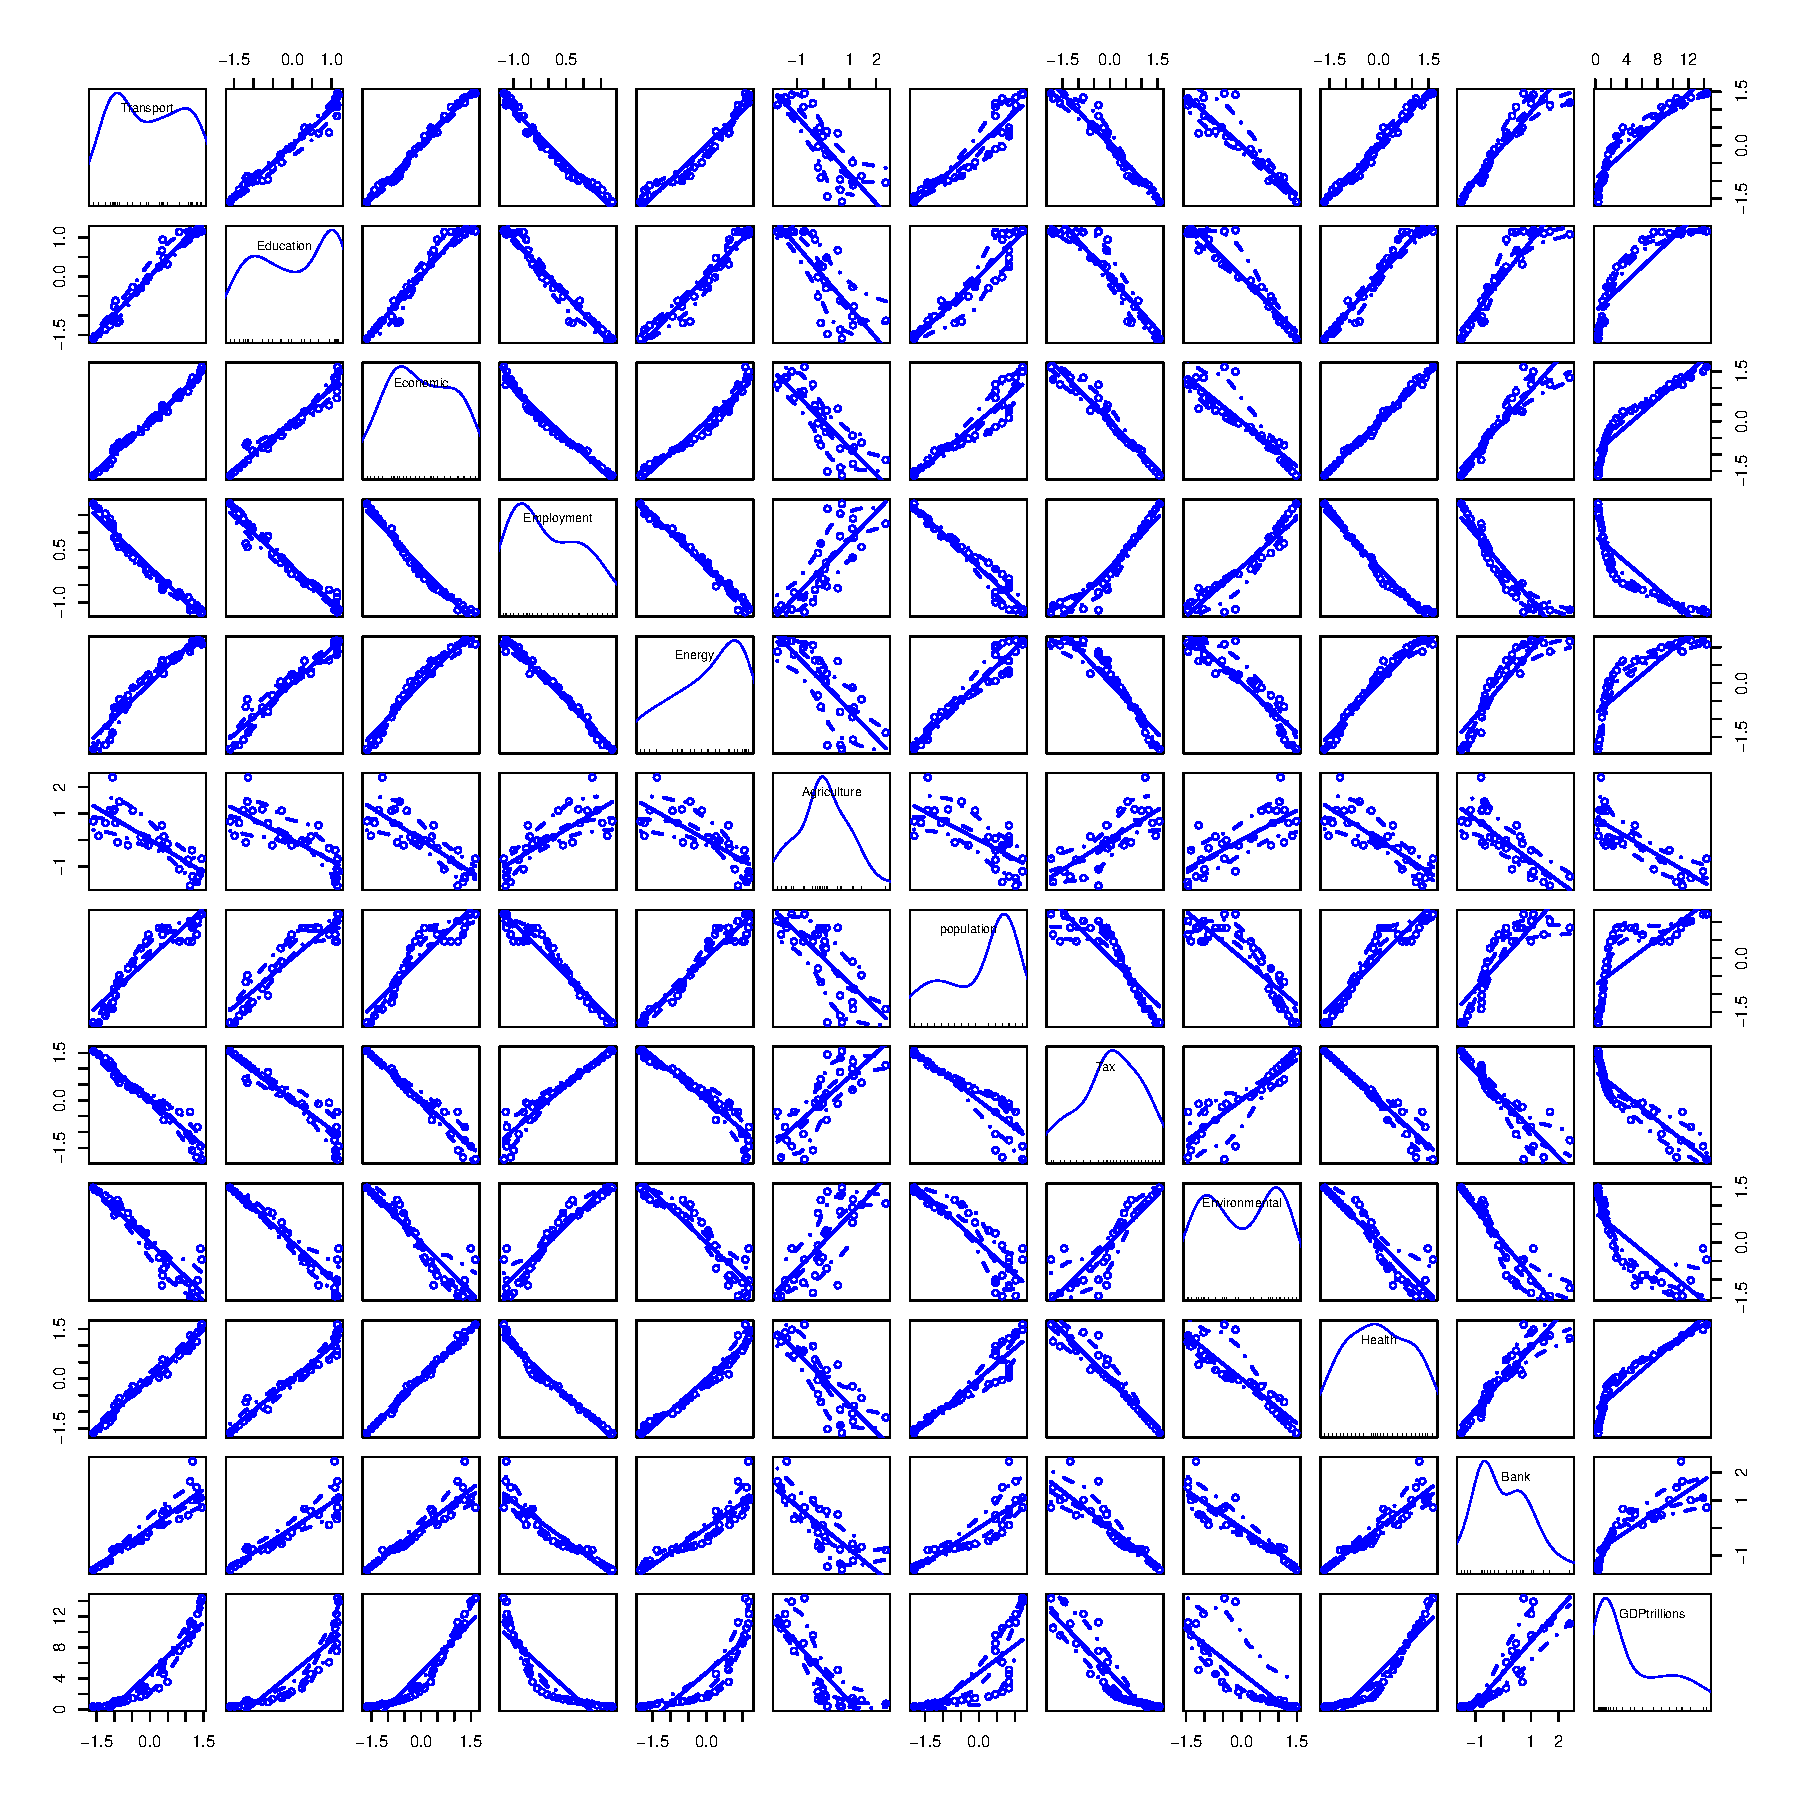
\includegraphics[width=\linewidth]{cor_cha2}
	\caption{correlations between variables}
\end{figure}

The corresponding Estimate, Std. Error, t value and Pr(>|t|) for the parameters to be evaluated are shown below. 
\begin{lstlisting}[language=r]
Residuals:
Min       1Q   Median       3Q      Max 
-0.69540 -0.23976  0.00536  0.12595  0.64783 

Coefficients:
Estimate Std. Error t value Pr(>|t|)    
(Intercept)    4.74032    0.06842  69.278  < 2e-16 ***
Transport      0.68066    0.73803   0.922 0.369296    
Education     -0.03972    0.55507  -0.072 0.943782    
Economic       7.75766    1.43442   5.408 4.71e-05 ***
Employment     7.38472    1.86038   3.969 0.000991 ***
Energy        -2.64365    0.62612  -4.222 0.000573 ***
Agriculture   -0.20557    0.12782  -1.608 0.126173    
population     0.24214    0.52034   0.465 0.647591    
Tax            0.69742    0.36268   1.923 0.071399 .  
Environmental -0.40180    0.39853  -1.008 0.327501    
Health         5.55964    1.14019   4.876 0.000142 ***
Bank           0.21679    0.28937   0.749 0.463995    
---
Signif. codes:  0 ‘***’ 0.001 ‘**’ 0.01 ‘*’ 0.05 ‘.’ 0.1 ‘ ’ 1

Residual standard error: 0.3685 on 17 degrees of freedom
Multiple R-squared:  0.9962,	Adjusted R-squared:  0.9937 
F-statistic: 403.5 on 11 and 17 DF,  p-value: < 2.2e-16
\end{lstlisting}

In the Pr(>|t|) column, you can see that the regression coefficients are significantly non-zero, indicating that for every change in each area, GDP would be expected to increase or decrease.

The R-squared term shows that the model can explain 99.82\% of the variance in body weight, which is also the sum of the actual and predicted values.

The standard error of the residuals is considered to be the average error of the model in predicting GDP using the principal components of each domain. F-statistics
The quantity tests whether all the predictor variables predict response variables above a certain probability level.

\subsubsection{Regression diagnosis}
\begin{lstlisting}[language=r]
> confint(ins_model)
                    2.5 %      97.5 %
(Intercept)    4.59595595  4.88468114
Transport     -0.87645502  2.23777954
Education     -1.21083028  1.13138070
Economic       4.73130412 10.78401945
Employment     3.45965552 11.30979064
Energy        -3.96465252 -1.32264413
Agriculture   -0.47524482  0.06409714
population    -0.85569042  1.33996772
Tax           -0.06776308  1.46259404
Environmental -1.24262867  0.43903682
Health         3.15404123  7.96523462
Bank          -0.39372703  0.82730015
\end{lstlisting}

For example, if Economy changes by 1\%, GDP will change within the 95\% confidence interval [4.73130412 , 10.78401945]; since the confidence interval for Transport contains 0, it can be concluded that the change in Transport is independent of GDP when all other variables are unchanged. 

However, your belief in these results is based on the premise that your data meet the statistical assumptions.

\begin{figure}[H]
	\centering
	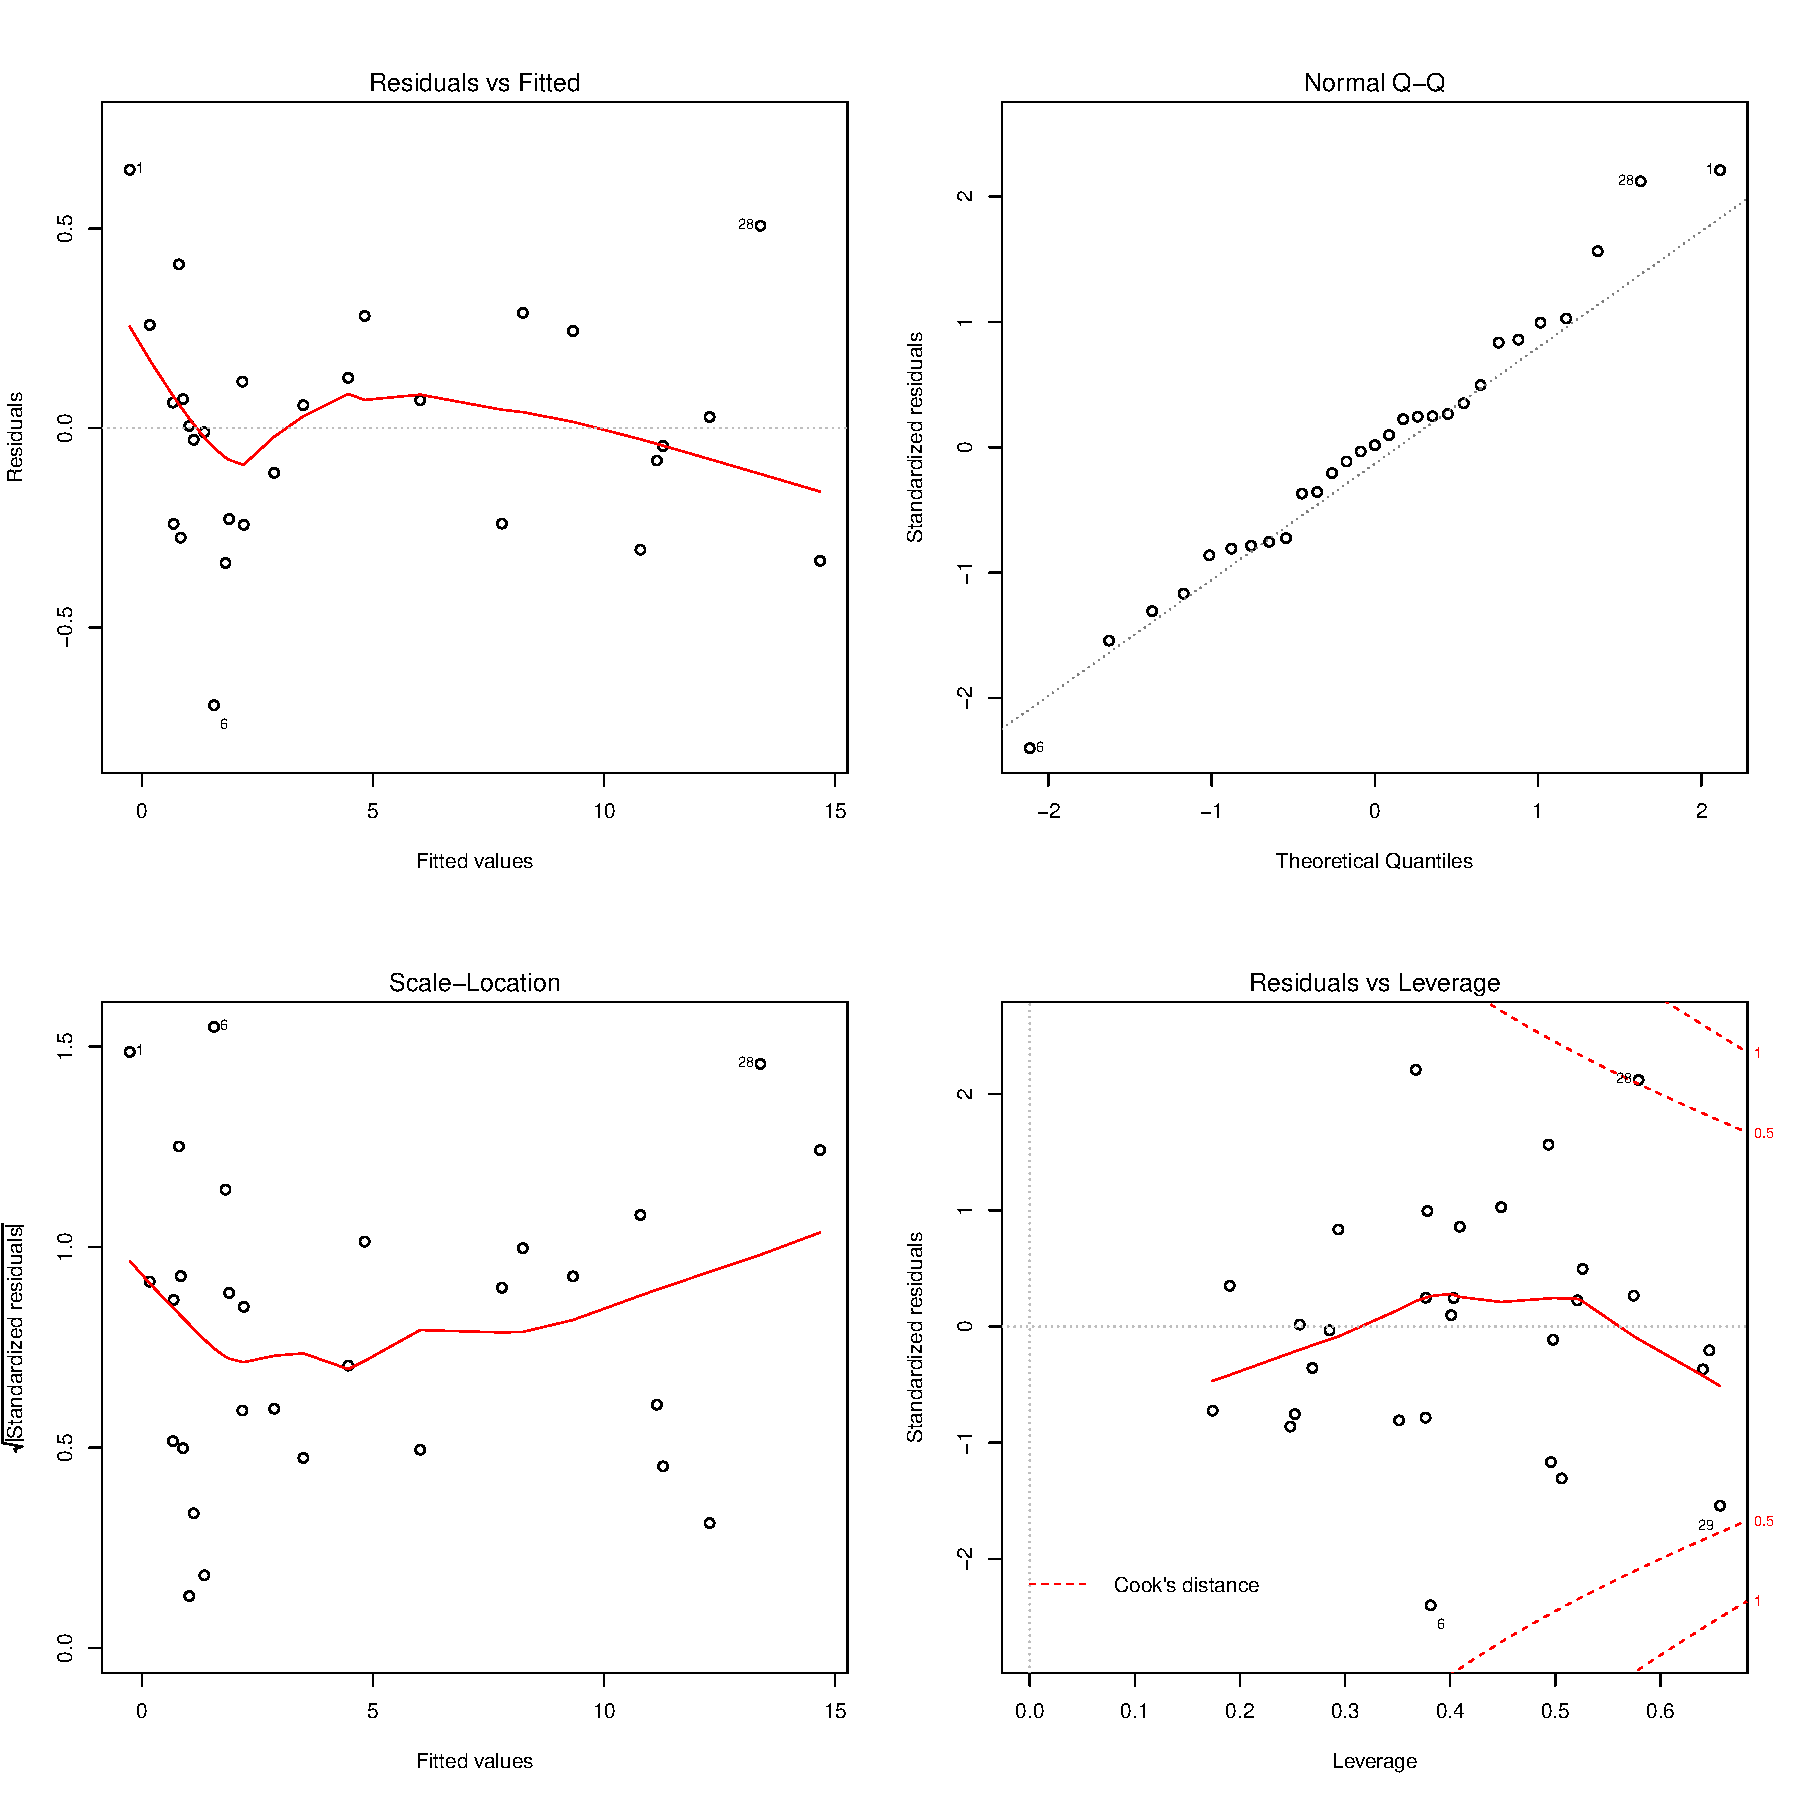
\includegraphics[width=0.7\linewidth]{四幅图_cha}
	\caption{Four graphs to evaluate the fit of the model}
\end{figure}

This second set of plots shows a good polynomial regression fit, which conforms to the assumptions of linearity, residual normality (except for observation 13) and homoskedasticity (constant residual variance).
%%%%%%%%%%%%%%%%%%%%%%%%%%%%%%%%%%%%%%%%%%%%%%%%%%%%%%%%%%%%%%

\section{Model Establishment and Solution of Problem 3}
Suggestions for economic countermeasures and policies in China in relevant areas.
\begin{itemize}
	\item As China's exports to the US will face more tariff barriers and the US will restrict the scientific and technological innovation capacity of Chinese enterprises in the name of strengthening the protection of intellectual property rights, our country should make use of its advantages and cooperate in various fields, including science and technology, to maximise its benefits. 
	\item With more restrictions on Chinese investment in the US, our country can expand market access and shift to a domestic-demand model of economic growth, which will provide more opportunities for US companies to participate in China's economic development and benefit from it.
	\item Rational resolution of bilateral trade frictions between China and the United States will promote the stability and development of economic relations and shape a new model of full cooperation and common development between the two countries in the 21st century.
	\item In response to the tax reform policy of the US, our country should improve the "camping reform" reform as soon as possible and achieve complete tax rebates for export products and services, so as to enhance the competitiveness of China's tax system.
	\item In view of China's lack of advantages in the high-end manufacturing industry, our country should attract foreign investment while maintaining the existing advantages in the middle and low-end manufacturing industry as far as possible, and at the same time increase the efforts to develop the high-end manufacturing industry.
	\item Follow the example of the USA and reduce the tax burden on businesses as a whole: lower the corporate tax rate. In addition, abolish and standardise deductions and preferential policies to improve the competitiveness of enterprises and establish a broad-based, low-tax corporate tax system. 
	\item Deepen reform and opening up and build a community of multilateral interests: in response to the changes in the global economic landscape influenced by the United States, turn pressure into motivation, build a modern economic system, and strengthen the comprehensive national power and economic innovation capacity.
	\item With regard to the immigration policy of the United States, our country should establish a database for tracking overseas talents based on the development needs of international students of different nationalities from the United States, taking into account their majors and other circumstances, and introduce relevant policies to attract overseas talents, so as to steadily promote the realisation of the strategic goal of a strong nation of talents.
\end{itemize}

%%%%%%%%%%%%%%%%%%%%%%%%%%%%%%%%%%%%%%%%%%%%%%%%%%%%%%%%%%%%%%%%%%%%%%%%%%%%%%%%%%%%%%%%%%%%%
\section{Strength and Weakness}
\subsection{Strength:}
\begin{itemize}
	\item Quantify different indicators and use principal component analysis to extract the principal components of multiple indicator variables for systematic analysis, which is easy to calculate and the results are simple and clear. 
	\item Take into account the actual situation of economic development of different countries to make the model more scientific and reasonable. 
	\item Organise and filter the collected data and use the reasonable data in solving equations. 
	4.Use multiple regression models to analyse predictive data, which is more persuasive and theoretical. 
	\item Using R to conduct textual analysis of the political positions and governance programmes of different candidates, this feature selection method is more scientific and persuasive.
\end{itemize}
\subsection{Weaknesses:}
\begin{itemize}
	\item The data collected is limited, the accuracy of the calculations is not high and the results obtained may differ from the actual situation. 
	\item When there are too many indicators, the statistical volume is large and the weights are difficult to determine, so there are certain errors.
\end{itemize}


%%%%%%%%%%%%%%%%%%%%%%%%%%%%%%%%%%%%%%%%%%%%%%%%%%%%%%%%%%%%%%%%%%%%%%%%%%%%%%%%%%%%%%%%%%%%%%%
\section{Future Work}

As just mentioned, one way of dealing with multicollinearity is to fit a different type of model (in this case, a ridge regression). In fact, if there are outliers and/or strong influence points, a robust regression model can be used instead of OLS regression. If the assumption of normality is violated, a non-parametric regression model can be used.

If there is significant non-linearity, a non-linear regression model can be attempted. If the assumption of error independence is violated, you can also use models that specialise in the structure of errors, such as time series models or multilevel regression models. 
 
Finally, we can also turn to the widely used generalised linear model, which can be applied to many OLS regression assumptions that do not work.
The case for a stand-up approach.

Judgements as to when the OLS regression fit needs to be improved and when a different approach is required are complex and rely on your knowledge of the subject matter to determine which model provides the best results.

%%%%%%%%%%%%%%%%%%%%%%%%%%%%%%%%%%%%%%%%%%%%%%%%%%%%%%%%%%%%%%%%%%%%%%%%%%%%%%%%%%%%%%%%%%%%%%
%参考文献
\begin{thebibliography}{9}%宽度9
\bibitem{1}\mbox{赵明强,林坚.西方经济学和统计学关于衡量经济发展的若干指标评介[J].统计研究},1989(01):69-73.
\bibitem{2} \mbox{黄慧群.关于完善衡量经济发展统计指标的思考[J].中国商贸,2014(33):155-157. }
\bibitem{3}\mbox{金春雨,张龙.美联储货币政策对中国经济的冲击[J].中国工业经济,2017(01):25-42.}
\bibitem{4}\mbox{张华,张素珍.美国紧缩性货币政策对中国省域经济的影响因素分析[J].湖北理工学院学报},2020,37
(06):33-39. 

\bibitem{5}\mbox{王青蓉. 函数型主成分分析及函数型线性回归模型的研究及应用[D].重庆工商大学,2020. }
\bibitem{6}\mbox{胡跃华,于石成.多重线性回归模型及其应用[J].中华预防医学杂志,2019(06):653-656.}
\bibitem{7}\mbox{闫达.基于 R 语言的自然语言文本预处理和统计学分析流程分析[J].西部皮革,2020,42(12):99+104.}
\end{thebibliography}

\newpage
%附录

\section{Appendix}
\subsection{Appendix A}
\begin{lstlisting}[language=r]
> library(psych)
> us02<- read.csv("E:/建模/yataibei2020/us/USA2_教育.csv",stringsAsFactors = FALSE)
> us022<-us02[,-1]

> pc<-principal(us022,nfactors = 1, score = T, rotate = "varimax")
Warning messages:
1: In cor.smooth(r) : Matrix was not positive definite, smoothing was done
2: In principal(us022, nfactors = 1, score = T, rotate = "varimax") :
The matrix is not positive semi-definite, scores found from Structure loadings

> pc
Principal Components Analysis
Call: principal(r = us022, nfactors = 1, rotate = "varimax", 
scores = T)
Standardized loadings (pattern matrix) based upon correlation matrix
PC1      h2   u2 com
中学教育.学生                           0.83 0.68086 0.32   1
中学教育.学生.女生所占百分比.          -0.20 0.04183 0.96   1
中学教育.一般学生                       0.82 0.67799 0.32   1
中学教育.一般学生.女生所占百分比.      -0.20 0.04197 0.96   1
中学师生比例                           -0.77 0.59577 0.40   1
入学率.中学.占总人数的百分比.           0.39 0.15291 0.85   1
入学率.中学.女生.占总人数的百分比.      0.26 0.06855 0.93   1
入学率.中学.男生.占总人数的百分比.      0.39 0.15230 0.85   1
入学率.中学.净百分比.                   0.41 0.17166 0.83   1
入学率.中学.女生.净百分比.              0.31 0.09846 0.90   1
入学率.中学.男生.净百分比.              0.23 0.05420 0.95   1
入学率.中学.私立.占中学总量的百分比.   -0.84 0.71104 0.29   1
中学教育.教师                           0.77 0.59226 0.41   1
中学教育.教师.女性                      0.84 0.69955 0.30   1
中学教育.教师..女性所占百分比.          0.88 0.78197 0.22   1
入学率.高等院校.占总人数的百分比.       0.81 0.64884 0.35   1
入学率.高等院校.女生.占总人数的百分比.  0.82 0.67557 0.32   1
入学率.高等院校.男生.占总人数的百分比.  0.75 0.56913 0.43   1
高等教育.教师..女性所占百分比.          0.81 0.65250 0.35   1
公共教育支出.总数.占政府支出的比例.    -0.21 0.04418 0.96   1
教育公共开支总额.总数.占GDP的比例.      0.72 0.52358 0.48   1
小学女生与男生的入学比例....           -0.01 0.00022 1.00   1
中小学女生与男生的入学比例...          -0.13 0.01742 0.98   1
中学女生与男生的入学比例...            -0.24 0.05612 0.94   1
高等学院女生与男生的入学比例....        0.69 0.47333 0.53   1
学校入学率.学前班.占总数的百分比.       0.48 0.22978 0.77   1
学校入学率.学前班.女生.占总数的百分比.  0.52 0.26978 0.73   1
学校入学率.学前班.男生.占总数的百分比.  0.46 0.21198 0.79   1
初等教育.小学生                         0.39 0.15392 0.85   1
初等教育.小学生.女生所占百分比.         0.11 0.01226 0.99   1
小学师生比例                           -0.77 0.59802 0.40   1
学校入学率.小学.占总数的百分比.        -0.85 0.72124 0.28   1
入学率.小学.女生.占总数的百分比.       -0.76 0.58169 0.42   1
入学率.小学.男生.占总数的百分比.       -0.83 0.68559 0.31   1
入学率.小学.净百分比.                  -0.92 0.84769 0.15   1
入学率.小学.女生.净百分比.             -0.88 0.78223 0.22   1
入学率.小学.男生.净百分比.             -0.91 0.83000 0.17   1
入学率.小学.私立.占总小学人数的百分比. -0.83 0.68093 0.32   1
初等教育.教师                           0.75 0.56217 0.44   1
初等教育.教师..女性所占百分比.          0.51 0.26164 0.74   1
小学总入学率.净比例.                   -0.76 0.58305 0.42   1
小学女生总入学率.净比例.               -0.70 0.48838 0.51   1
小学男生总入学率.净比例.               -0.80 0.63695 0.36   1
失学儿童.小学                           0.86 0.74817 0.25   1
失学女童.小学                           0.81 0.65031 0.35   1
失学男童.小学                           0.89 0.79152 0.21   1

PC1
SS loadings    20.51
Proportion Var  0.45

Mean item complexity =  1
Test of the hypothesis that 1 component is sufficient.

The root mean square of the residuals (RMSR) is  0.23 
with the empirical chi square  2456.07  with prob <  7.3e-126 

Fit based upon off diagonal values = 0.79> #提取主成分。psych包中的principal( )函数可以根据原始数据或相关系数矩阵做主成分分析,其使用格式为:

> round(unclass(pc$weights),2) ## 获取主成分得分的系数。
PC1
中学教育.学生                           0.83
中学教育.学生.女生所占百分比.          -0.20
中学教育.一般学生                       0.82
中学教育.一般学生.女生所占百分比.      -0.20
中学师生比例                           -0.77
入学率.中学.占总人数的百分比.           0.39
入学率.中学.女生.占总人数的百分比.      0.26
入学率.中学.男生.占总人数的百分比.      0.39
入学率.中学.净百分比.                   0.41
入学率.中学.女生.净百分比.              0.31
入学率.中学.男生.净百分比.              0.23
入学率.中学.私立.占中学总量的百分比.   -0.84
中学教育.教师                           0.77
中学教育.教师.女性                      0.84
中学教育.教师..女性所占百分比.          0.88
入学率.高等院校.占总人数的百分比.       0.81
入学率.高等院校.女生.占总人数的百分比.  0.82
入学率.高等院校.男生.占总人数的百分比.  0.75
高等教育.教师..女性所占百分比.          0.81
公共教育支出.总数.占政府支出的比例.    -0.21
教育公共开支总额.总数.占GDP的比例.      0.72
小学女生与男生的入学比例....           -0.01
中小学女生与男生的入学比例...          -0.13
中学女生与男生的入学比例...            -0.24
高等学院女生与男生的入学比例....        0.69
学校入学率.学前班.占总数的百分比.       0.48
学校入学率.学前班.女生.占总数的百分比.  0.52
学校入学率.学前班.男生.占总数的百分比.  0.46
初等教育.小学生                         0.39
初等教育.小学生.女生所占百分比.         0.11
小学师生比例                           -0.77
学校入学率.小学.占总数的百分比.        -0.85
入学率.小学.女生.占总数的百分比.       -0.76
入学率.小学.男生.占总数的百分比.       -0.83
入学率.小学.净百分比.                  -0.92
入学率.小学.女生.净百分比.             -0.88
入学率.小学.男生.净百分比.             -0.91
入学率.小学.私立.占总小学人数的百分比. -0.83
初等教育.教师                           0.75
初等教育.教师..女性所占百分比.          0.51
小学总入学率.净比例.                   -0.76
小学女生总入学率.净比例.               -0.70
小学男生总入学率.净比例.               -0.80
失学儿童.小学                           0.86
失学女童.小学                           0.81
失学男童.小学                           0.89

 \end{lstlisting}
\subsection{Appendix B}
\begin{lstlisting}[language=matlab]
Clear,clc
A=load('USA10_医疗.csv');
B=load('us10new.txt');
C=A*B;
xlswrite('U10_医疗.csv',C)%把计算结果写入excel中
\end{lstlisting}
\subsection{Appendix C}
\begin{lstlisting}[language=r]
> library(psych)
> us01<- read.csv("E:/建模/yataibei2020/data2.0/USA1_交通_网络.csv",stringsAsFactors = FALSE)
> us011<-us1[,-1]

> pc<-principal(us011, nfactors = 1, score = T, rotate = "varimax")
> pc
Principal Components Analysis
Call: principal(r = us011, nfactors = 1, rotate = "varimax", 
scores = T)
Standardized loadings (pattern matrix) based upon correlation matrix
PC1      h2    u2 com
航空运输量.注册承运人全球出港量             0.96 9.2e-01 0.078   1
航空运输.货运量.百万吨.公里.                0.99 9.8e-01 0.015   1
航空运输.客运量                             0.98 9.5e-01 0.045   1
道路部门燃料消耗量.千吨石油当量.            0.99 9.8e-01 0.022   1
道路部门人均燃料消耗量.千吨石油当量.        0.98 9.5e-01 0.046   1
道路部门能源消耗量.千吨石油当量.            0.99 9.9e-01 0.014   1
道路部门人均能源消耗量.千吨石油当量.        0.80 6.5e-01 0.353   1
道路部门能源消耗量.占总能源消耗量的百分比.  0.96 9.3e-01 0.071   1
公路货运量..百万吨.公里.                    0.98 9.5e-01 0.048   1
道路部门汽油消耗量.千吨石油当量.            0.95 8.9e-01 0.106   1
道路部门人均汽油消耗量.千吨石油当量.        0.00 5.3e-06 1.000   1
公路网络总量.百分比.                        0.93 8.6e-01 0.144   1
铁路货运量.百万吨.公里.                     0.98 9.6e-01 0.039   1
铁路.总公里数.                             -0.01 3.1e-05 1.000   1
移动蜂窝式无线通讯系统的电话租用            0.93 8.6e-01 0.143   1
移动蜂窝式无线通讯系统的电话租用.每百人.    0.94 8.8e-01 0.118   1
电话线路                                    0.67 4.5e-01 0.548   1
每100人所拥有的电话线路数量                 0.21 4.4e-02 0.956   1
互联网用户.每.100.人.                       0.97 9.4e-01 0.055   1

PC1
SS loadings    14.20
Proportion Var  0.75

Mean item complexity =  1
Test of the hypothesis that 1 component is sufficient.

The root mean square of the residuals (RMSR) is  0.18 
with the empirical chi square  329.8  with prob <  3.5e-15 

Fit based upon off diagonal values = 0.94

> round(unclass(pc$weights),2)
PC1
航空运输量.注册承运人全球出港量            0.07
航空运输.货运量.百万吨.公里.               0.07
航空运输.客运量                            0.07
道路部门燃料消耗量.千吨石油当量.           0.07
道路部门人均燃料消耗量.千吨石油当量.       0.07
道路部门能源消耗量.千吨石油当量.           0.07
道路部门人均能源消耗量.千吨石油当量.       0.06
道路部门能源消耗量.占总能源消耗量的百分比. 0.07
公路货运量..百万吨.公里.                   0.07
道路部门汽油消耗量.千吨石油当量.           0.07
道路部门人均汽油消耗量.千吨石油当量.       0.00
公路网络总量.百分比.                       0.07
铁路货运量.百万吨.公里.                    0.07
铁路.总公里数.                             0.00
移动蜂窝式无线通讯系统的电话租用           0.07
移动蜂窝式无线通讯系统的电话租用.每百人.   0.07
电话线路                                   0.05
每100人所拥有的电话线路数量                0.01
互联网用户.每.100.人.                      0.07 
\end{lstlisting}
\subsection{Appendix D}
\begin{lstlisting}[language=r]
> usa<-read.csv("E:/建模/yataibei2020/主成分分析值 美国_new/us合并.csv",stringsAsFactors = FALSE)
> View(usa)
> usa_z<-as.data.frame(scale(usa[-1]))
> write.table(usa_z,"E:/建模/yataibei2020/主成分分析值 美国_new/us合并_Z.csv",row.names=FALSE, col.names=TRUE, sep="," )

> data<-read.csv("E:/建模/yataibei2020/主成分分析值 美国_new/us合并_Z.csv",stringsAsFactors = FALSE)
> data<-as.data.frame(data[,-1])

> ins_model <- lm(data$GDPtrillions ~ ., data = data)
> ins_model

Call:
lm(formula = data$GDPtrillions ~ ., data = data)

Coefficients:
(Intercept)      Transport      Education       Economic     Employment         Energy  
12.93310        0.69428       -0.50169        5.18329        1.44506       -1.69210  
Agriculture     population            Tax  Environmental         Health           Bank  
-0.05023        1.62642        1.59604        0.11109        1.47196       -0.16434 

> summary(ins_model)

Call:
lm(formula = data$GDPtrillions ~ ., data = data)

Residuals:
Min       1Q   Median       3Q      Max 
-0.44285 -0.13036  0.04252  0.09040  0.31347 

Coefficients:
Estimate Std. Error t value Pr(>|t|)    
(Intercept)   12.93310    0.04539 284.918  < 2e-16 ***
Transport      0.69428    0.48961   1.418 0.174253    
Education     -0.50169    0.36823  -1.362 0.190842    
Economic       5.18329    0.95159   5.447 4.35e-05 ***
Employment     1.44506    1.23417   1.171 0.257800    
Energy        -1.69210    0.41537  -4.074 0.000790 ***
Agriculture   -0.05023    0.08479  -0.592 0.561410    
population     1.62642    0.34519   4.712 0.000201 ***
Tax            0.59604    0.24060   2.477 0.024036 *  
Environmental  0.11109    0.26439   0.420 0.679605    
Health         1.47196    0.75640   1.946 0.068377 .  
Bank          -0.16434    0.19197  -0.856 0.403851    
---
Signif. codes:  0 ‘***’ 0.001 ‘**’ 0.01 ‘*’ 0.05 ‘.’ 0.1 ‘ ’ 1

Residual standard error: 0.2444 on 17 degrees of freedom
Multiple R-squared:  0.9982,	Adjusted R-squared:  0.9971 
F-statistic: 867.1 on 11 and 17 DF,  p-value: < 2.2e-16
=============================================================

> library(car)
> scatterplotMatrix(data,spread=FALSE,lty.smooth=2)



==============================================================
> confint(ins_model)
2.5 %     97.5 %
(Intercept)   12.8373336 13.0288729
Transport     -0.3387061  1.7272661
Education     -1.2785997  0.2752149
Economic       3.1756110  7.1909611
Employment    -1.1588123  4.0489398
Energy        -2.5684494 -0.8157504
Agriculture   -0.2291266  0.1286709
population     0.8981248  2.3547166
Tax            0.0884219  1.1036554
Environmental -0.4467115  0.6688995
Health        -0.1239006  3.0678281
Bank          -0.5693537  0.2406715     


============================================================
> par(mfrow=c(2,2))
> plot(ins_model)

\end{lstlisting}
\subsection{Appendix E}
\begin{lstlisting}[language=r]
> data<-read.csv("E:/建模/yataibei2020/主成分分析值 中国/us合并ccccccc_Z.csv",stringsAsFactors = FALSE)
> data<-as.data.frame(data[,-1])
> 
> ins_model <- lm(data$GDPtrillions ~ ., data = data)
> ins_model

Call:
lm(formula = data$GDPtrillions ~ ., data = data)

Coefficients:
(Intercept)      Transport      Education       Economic     Employment         Energy  
4.74032        0.68066       -0.03972        7.75766        7.38472       -2.64365  
Agriculture     population            Tax  Environmental         Health           Bank  
-0.20557        0.24214        0.69742       -0.40180        5.55964        0.21679  

> summary(ins_model)

Call:
lm(formula = data$GDPtrillions ~ ., data = data)

Residuals:
Min       1Q   Median       3Q      Max 
-0.69540 -0.23976  0.00536  0.12595  0.64783 

Coefficients:
Estimate Std. Error t value Pr(>|t|)    
(Intercept)    4.74032    0.06842  69.278  < 2e-16 ***
Transport      0.68066    0.73803   0.922 0.369296    
Education     -0.03972    0.55507  -0.072 0.943782    
Economic       7.75766    1.43442   5.408 4.71e-05 ***
Employment     7.38472    1.86038   3.969 0.000991 ***
Energy        -2.64365    0.62612  -4.222 0.000573 ***
Agriculture   -0.20557    0.12782  -1.608 0.126173    
population     0.24214    0.52034   0.465 0.647591    
Tax            0.69742    0.36268   1.923 0.071399 .  
Environmental -0.40180    0.39853  -1.008 0.327501    
Health         5.55964    1.14019   4.876 0.000142 ***
Bank           0.21679    0.28937   0.749 0.463995    
---
Signif. codes:  0 ‘***’ 0.001 ‘**’ 0.01 ‘*’ 0.05 ‘.’ 0.1 ‘ ’ 1

Residual standard error: 0.3685 on 17 degrees of freedom
Multiple R-squared:  0.9962,	Adjusted R-squared:  0.9937 
F-statistic: 403.5 on 11 and 17 DF,  p-value: < 2.2e-16
=========================================================================
> 
> pairs(data[c("Transport", "Education", "Economic","Employment","Energy","Agriculture","population",
+                   "Tax","Environmental","Health","Bank")])

> confint(ins_model)
2.5 %      97.5 %
(Intercept)    4.59595595  4.88468114
Transport     -0.87645502  2.23777954
Education     -1.21083028  1.13138070
Economic       4.73130412 10.78401945
Employment     3.45965552 11.30979064
Energy        -3.96465252 -1.32264413
Agriculture   -0.47524482  0.06409714
population    -0.85569042  1.33996772
Tax           -0.06776308  1.46259404
Environmental -1.24262867  0.43903682
Health         3.15404123  7.96523462
Bank          -0.39372703  0.82730015
There were 50 or more warnings (use warnings() to see the first 50)
> par(mfrow=c(2,2))
> plot(ins_model)
\end{lstlisting}
\subsection{Appendix F}
\begin{lstlisting}[language=r]
> DT<-read.csv("E:/建模/yataibei2020/DonaldTweets.csv",stringsAsFactors = FALSE)
> str(DT)
'data.frame':	7375 obs. of  2 variables:
$ Date      : chr  "2016.11.11" "2016.11.11" "2016.11.11" "2016.11.11" ...
$ Tweet_Text: chr  "Today we express our deepest gratitude to all those who have served in our armed forces. #ThankAVet https://t.co/wPk7QWpK8Z" "Busy day planned in New York. Will soon be making some very important decisions on the people who will be runni"| __truncated__ "Love the fact that the small groups of protesters last night have passion for our great country. We will all co"| __truncated__ "Just had a very open and successful presidential election. Now professional protesters, incited by the media, a"| __truncated__ ...
> library(tm)
> DT_corpus<-VCorpus(VectorSource(DT$Tweet_Text))
> print(DT_corpus)
<<VCorpus>>
Metadata:  corpus specific: 0, document level (indexed): 0
Content:  documents: 7375
> inspect(DT_corpus[1:3])
<<VCorpus>>
Metadata:  corpus specific: 0, document level (indexed): 0
Content:  documents: 3

[[1]]
<<PlainTextDocument>>
Metadata:  7
Content:  chars: 123

[[2]]
<<PlainTextDocument>>
Metadata:  7
Content:  chars: 129

[[3]]
<<PlainTextDocument>>
Metadata:  7
Content:  chars: 136

> corpus_clean<-tm_map(DT_corpus,tolower)
> corpus_clean<-tm_map(corpus_clean, removeNumbers)
> corpus_clean<-tm_map(corpus_clean, removeWords , stopwords())
> corpus_clean<-tm_map(corpus_clean, removePunctuation)
> corpus_clean<-tm_map(corpus_clean, stripWhitespace)
> inspect(corpus_clean[1:3])
<<VCorpus>>
Metadata:  corpus specific: 0, document level (indexed): 0
Content:  documents: 3

[[1]]
[1] today express deepest gratitude served armed forces thankavet httpstcowpkqwpkz

[[2]]
[1] busy day planned new york will soon making important decisions people will running government

[[3]]
[1] love fact small groups protesters last night passion great country will come together proud

> corpus_clean<-tm_map(corpus_clean, PlainTextDocument)
> BT_dtm<-DocumentTermMatrix(corpus_clean)
> library(wordcloud)
> wordcloud(corpus_clean, min.freq =0,random.order = FALSE)
\end{lstlisting}

\end{document} 